\documentclass[twoside]{book}

% Packages required by doxygen
\usepackage{fixltx2e}
\usepackage{calc}
\usepackage{doxygen}
\usepackage[export]{adjustbox} % also loads graphicx
\usepackage{graphicx}
\usepackage[utf8]{inputenc}
\usepackage{makeidx}
\usepackage{multicol}
\usepackage{multirow}
\PassOptionsToPackage{warn}{textcomp}
\usepackage{textcomp}
\usepackage[nointegrals]{wasysym}
\usepackage[table]{xcolor}

% NLS support packages
\usepackage[french]{babel}

% Font selection
\usepackage[T1]{fontenc}
\usepackage[scaled=.90]{helvet}
\usepackage{courier}
\usepackage{amssymb}
\usepackage{sectsty}
\renewcommand{\familydefault}{\sfdefault}
\allsectionsfont{%
  \fontseries{bc}\selectfont%
  \color{darkgray}%
}
\renewcommand{\DoxyLabelFont}{%
  \fontseries{bc}\selectfont%
  \color{darkgray}%
}
\newcommand{\+}{\discretionary{\mbox{\scriptsize$\hookleftarrow$}}{}{}}

% Page & text layout
\usepackage{geometry}
\geometry{%
  a4paper,%
  top=2.5cm,%
  bottom=2.5cm,%
  left=2.5cm,%
  right=2.5cm%
}
\tolerance=750
\hfuzz=15pt
\hbadness=750
\setlength{\emergencystretch}{15pt}
\setlength{\parindent}{0cm}
\setlength{\parskip}{3ex plus 2ex minus 2ex}
\makeatletter
\renewcommand{\paragraph}{%
  \@startsection{paragraph}{4}{0ex}{-1.0ex}{1.0ex}{%
    \normalfont\normalsize\bfseries\SS@parafont%
  }%
}
\renewcommand{\subparagraph}{%
  \@startsection{subparagraph}{5}{0ex}{-1.0ex}{1.0ex}{%
    \normalfont\normalsize\bfseries\SS@subparafont%
  }%
}
\makeatother

% Headers & footers
\usepackage{fancyhdr}
\pagestyle{fancyplain}
\fancyhead[LE]{\fancyplain{}{\bfseries\thepage}}
\fancyhead[CE]{\fancyplain{}{}}
\fancyhead[RE]{\fancyplain{}{\bfseries\leftmark}}
\fancyhead[LO]{\fancyplain{}{\bfseries\rightmark}}
\fancyhead[CO]{\fancyplain{}{}}
\fancyhead[RO]{\fancyplain{}{\bfseries\thepage}}
\fancyfoot[LE]{\fancyplain{}{}}
\fancyfoot[CE]{\fancyplain{}{}}
\fancyfoot[RE]{\fancyplain{}{\bfseries\scriptsize Généré par Doxygen }}
\fancyfoot[LO]{\fancyplain{}{\bfseries\scriptsize Généré par Doxygen }}
\fancyfoot[CO]{\fancyplain{}{}}
\fancyfoot[RO]{\fancyplain{}{}}
\renewcommand{\footrulewidth}{0.4pt}
\renewcommand{\chaptermark}[1]{%
  \markboth{#1}{}%
}
\renewcommand{\sectionmark}[1]{%
  \markright{\thesection\ #1}%
}

% Indices & bibliography
\usepackage{natbib}
\usepackage[titles]{tocloft}
\setcounter{tocdepth}{3}
\setcounter{secnumdepth}{5}
\makeindex

% Hyperlinks (required, but should be loaded last)
\usepackage{ifpdf}
\ifpdf
  \usepackage[pdftex,pagebackref=true]{hyperref}
\else
  \usepackage[ps2pdf,pagebackref=true]{hyperref}
\fi
\hypersetup{%
  colorlinks=true,%
  linkcolor=blue,%
  citecolor=blue,%
  unicode%
}

% Custom commands
\newcommand{\clearemptydoublepage}{%
  \newpage{\pagestyle{empty}\cleardoublepage}%
}

\usepackage{caption}
\captionsetup{labelsep=space,justification=centering,font={bf},singlelinecheck=off,skip=4pt,position=top}

%===== C O N T E N T S =====

\begin{document}

% Titlepage & ToC
\hypersetup{pageanchor=false,
             bookmarksnumbered=true,
             pdfencoding=unicode
            }
\pagenumbering{alph}
\begin{titlepage}
\vspace*{7cm}
\begin{center}%
{\Large Solveur Elements Finis/\+Skyline Matrix \\[1ex]\large 1.\+0 }\\
\vspace*{1cm}
{\large Généré par Doxygen 1.8.13}\\
\end{center}
\end{titlepage}
\clearemptydoublepage
\pagenumbering{roman}
\tableofcontents
\clearemptydoublepage
\pagenumbering{arabic}
\hypersetup{pageanchor=true}

%--- Begin generated contents ---
\chapter{Utilisation de matrice S\+K\+Y\+L\+I\+NE et de la décomposition de Cholesky pour la résolution d\textquotesingle{}un problème d\textquotesingle{}éléments finis}
\label{index}\hypertarget{index}{}\hypertarget{index_Présentation}{}\section{Présentation}\label{index_Présentation}
On utilise des matrices S\+K\+Y\+L\+I\+NE pour représenter les matrices en mémoires. On peut alors en calculer une décomposition de Cholesky. Enfin, on peut résoudre le problème d\textquotesingle{}élément finis. \hypertarget{index_Cholesky}{}\section{Cholesky}\label{index_Cholesky}
Ici on ne stocke pas la matrice L calculé, mais sa transposée. Cela permet de n\textquotesingle{}avoir a gérer que des acces en ligne durant les phases d\textquotesingle{}écriture. \hypertarget{index_SOLVER}{}\section{S\+O\+L\+V\+ER}\label{index_SOLVER}
Il faut modifier A(x) et F(x) pour résoudre le problème voulu. \hypertarget{index_Compilation}{}\section{Compilation}\label{index_Compilation}
Pour compiler le code executer le script {\itshape compile.\+sh}. 
\chapter{Index des modules}
\section{Liste des modules}
Liste de tous les modules avec une brève description \+:\begin{DoxyCompactList}
\item\contentsline{section}{\hyperlink{namespacecholesky__mod}{cholesky\+\_\+mod} \\*Ce module permet de calculer la décomposition de Cholesky d\textquotesingle{}une matrice définie positive }{\pageref{namespacecholesky__mod}}{}
\item\contentsline{section}{\hyperlink{namespaceskyline}{skyline} \\*Ce module permet de stocker une matrice sous la forme d\textquotesingle{}une matrice Skyline (profil) }{\pageref{namespaceskyline}}{}
\item\contentsline{section}{\hyperlink{namespacesolver}{solver} \\*Ce module permet de résoudre un problème d\textquotesingle{}éléments fini }{\pageref{namespacesolver}}{}
\end{DoxyCompactList}

\chapter{Index du type de données}
\section{Liste des types de données}
Liste des types de données avec une brève description \+:\begin{DoxyCompactList}
\item\contentsline{section}{\hyperlink{structskyline_1_1skyline__matrix}{skyline\+::skyline\+\_\+matrix} }{\pageref{structskyline_1_1skyline__matrix}}{}
\end{DoxyCompactList}

\chapter{Index des fichiers}
\section{Liste des fichiers}
Liste de tous les fichiers avec une brève description \+:\begin{DoxyCompactList}
\item\contentsline{section}{src/\hyperlink{_c_h_o_l_e_s_k_y_8f90}{C\+H\+O\+L\+E\+S\+K\+Y.\+f90} }{\pageref{_c_h_o_l_e_s_k_y_8f90}}{}
\item\contentsline{section}{src/\hyperlink{main_8f90}{main.\+f90} }{\pageref{main_8f90}}{}
\item\contentsline{section}{src/\hyperlink{_s_k_y_l_i_n_e_8f90}{S\+K\+Y\+L\+I\+N\+E.\+f90} }{\pageref{_s_k_y_l_i_n_e_8f90}}{}
\item\contentsline{section}{src/\hyperlink{_s_o_l_v_e_r_8f90}{S\+O\+L\+V\+E\+R.\+f90} }{\pageref{_s_o_l_v_e_r_8f90}}{}
\end{DoxyCompactList}

\chapter{Documentation des modules}
\hypertarget{namespacecholesky__mod}{}\section{cholesky\+\_\+mod Module Reference}
\label{namespacecholesky__mod}\index{cholesky\+\_\+mod@{cholesky\+\_\+mod}}


Ce module permet de calculer la décomposition de Cholesky d\textquotesingle{}une matrice définie positive.  


\subsection*{Functions/\+Subroutines}
\begin{DoxyCompactItemize}
\item 
type(skyline\+\_\+matrix) function \hyperlink{namespacecholesky__mod_a1cbaf08b2c159febf9d4a76d7819a1cd}{cholesky} (M)
\begin{DoxyCompactList}\small\item\em Calcule la décompostion de Cholesky d\textquotesingle{}une matrice de type S\+K\+Y\+L\+I\+NE. \end{DoxyCompactList}\end{DoxyCompactItemize}


\subsection{Detailed Description}
Ce module permet de calculer la décomposition de Cholesky d\textquotesingle{}une matrice définie positive. 

\begin{DoxyAuthor}{Author}
Kara Abdelhadi, Mechineau Alexandre 
\end{DoxyAuthor}


\subsection{Function/\+Subroutine Documentation}
\mbox{\Hypertarget{namespacecholesky__mod_a1cbaf08b2c159febf9d4a76d7819a1cd}\label{namespacecholesky__mod_a1cbaf08b2c159febf9d4a76d7819a1cd}} 
\index{cholesky\+\_\+mod@{cholesky\+\_\+mod}!cholesky@{cholesky}}
\index{cholesky@{cholesky}!cholesky\+\_\+mod@{cholesky\+\_\+mod}}
\subsubsection{\texorpdfstring{cholesky()}{cholesky()}}
{\footnotesize\ttfamily type(skyline\+\_\+matrix) function cholesky\+\_\+mod\+::cholesky (\begin{DoxyParamCaption}\item[{type(skyline\+\_\+matrix)}]{M }\end{DoxyParamCaption})}



Calcule la décompostion de Cholesky d\textquotesingle{}une matrice de type S\+K\+Y\+L\+I\+NE. 


\begin{DoxyParams}{Parameters}
{\em M} & Matrice S\+K\+Y\+L\+I\+NE \\
\hline
\end{DoxyParams}
\begin{DoxyReturn}{Returns}
Matrice S\+K\+Y\+L\+I\+NE triangulaire supérieure contenant la décomposition 
\end{DoxyReturn}
Here is the call graph for this function\+:\nopagebreak
\begin{figure}[H]
\begin{center}
\leavevmode
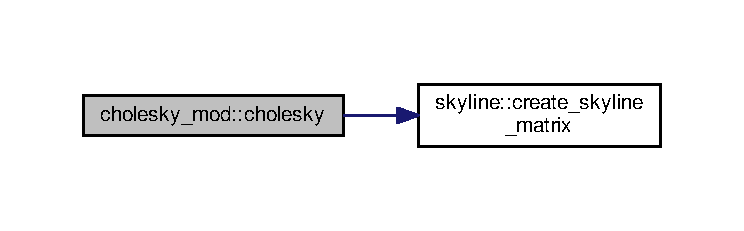
\includegraphics[width=350pt]{namespacecholesky__mod_a1cbaf08b2c159febf9d4a76d7819a1cd_cgraph}
\end{center}
\end{figure}
Here is the caller graph for this function\+:\nopagebreak
\begin{figure}[H]
\begin{center}
\leavevmode
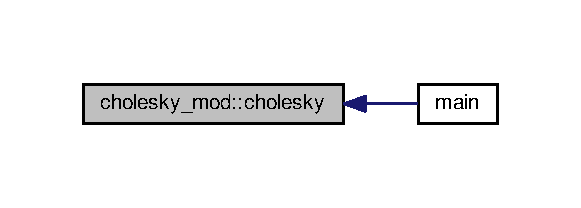
\includegraphics[width=279pt]{namespacecholesky__mod_a1cbaf08b2c159febf9d4a76d7819a1cd_icgraph}
\end{center}
\end{figure}

\hypertarget{namespaceskyline}{}\section{skyline Module Reference}
\label{namespaceskyline}\index{skyline@{skyline}}


Ce module permet de stocker une matrice sous la forme d\textquotesingle{}une matrice Skyline (profil)  


\subsection*{Data Types}
\begin{DoxyCompactItemize}
\item 
type \hyperlink{structskyline_1_1skyline__matrix}{skyline\+\_\+matrix}
\end{DoxyCompactItemize}
\subsection*{Functions/\+Subroutines}
\begin{DoxyCompactItemize}
\item 
type(\hyperlink{structskyline_1_1skyline__matrix}{skyline\+\_\+matrix}) function \hyperlink{namespaceskyline_a5fe1d351df2e3a07f96028d1d2a892a8}{create\+\_\+skyline\+\_\+matrix} (m, n)
\begin{DoxyCompactList}\small\item\em Créé une matrice S\+K\+Y\+L\+I\+NE vide de dimension $(m,n)$. \end{DoxyCompactList}\item 
type(\hyperlink{structskyline_1_1skyline__matrix}{skyline\+\_\+matrix}) function \hyperlink{namespaceskyline_a86a4fe28bc106ef42d25cf7596c108bf}{create\+\_\+skyline\+\_\+matrix\+\_\+from\+\_\+file} (filename)
\begin{DoxyCompactList}\small\item\em Créé une matrice S\+K\+Y\+L\+I\+NE depuis les données contenus dans un fichier. \end{DoxyCompactList}\item 
subroutine \hyperlink{namespaceskyline_a3377a8391ad2d61659689fc8c4130bdc}{write\+\_\+skyline\+\_\+matrix\+\_\+to\+\_\+file} (M, filename)
\begin{DoxyCompactList}\small\item\em Sauvegarde une matrice S\+K\+Y\+L\+I\+NE dans un fichier. \end{DoxyCompactList}\item 
subroutine \hyperlink{namespaceskyline_a583c70b26e3bcb37ecb679f5c11ec2f4}{free\+\_\+skyline\+\_\+matrix} (M)
\begin{DoxyCompactList}\small\item\em Supprime les allocations mémoires d\textquotesingle{}une matrice S\+K\+Y\+L\+I\+NE. \end{DoxyCompactList}\item 
real function \hyperlink{namespaceskyline_a28077ec6714b830771f90da1b674b0ce}{get} (M, row, col)
\begin{DoxyCompactList}\small\item\em Accède aux éléments d\textquotesingle{}une matrice S\+K\+Y\+L\+I\+NE. \end{DoxyCompactList}\item 
integer function \hyperlink{namespaceskyline_a25b1e027d99abb67ab844d7b657a5843}{position\+\_\+on\+\_\+s} (M, row, col)
\begin{DoxyCompactList}\small\item\em Calcule la position d\textquotesingle{}un élément dans le tableau stockant les données. \end{DoxyCompactList}\item 
integer function \hyperlink{namespaceskyline_a9f07218be321c12bea1d84f6b629e346}{number\+\_\+item\+\_\+on\+\_\+line} (M, row)
\begin{DoxyCompactList}\small\item\em Calcule le nombre d\textquotesingle{}élément stocké sur une ligne. \end{DoxyCompactList}\item 
subroutine \hyperlink{namespaceskyline_a428818245223fbf6e3a5a2264f8f1a65}{display} (M)
\begin{DoxyCompactList}\small\item\em Affiche une matrice S\+K\+Y\+L\+I\+NE. \end{DoxyCompactList}\item 
subroutine \hyperlink{namespaceskyline_aedb0d55aecd5f4cae4dc3593a5e89f0f}{display\+\_\+debug} (M)
\begin{DoxyCompactList}\small\item\em Affiche des informations de debuguage d\textquotesingle{}une matrice S\+K\+Y\+L\+I\+NE. \end{DoxyCompactList}\item 
real function, dimension(\+:), allocatable \hyperlink{namespaceskyline_ae156a973c4a30bd2740af6ef2fdfa1d9}{prod\+\_\+mat\+\_\+vec} (M, X)
\begin{DoxyCompactList}\small\item\em Calcule Le produit entre une matrice et un vecteur. \end{DoxyCompactList}\end{DoxyCompactItemize}


\subsection{Detailed Description}
Ce module permet de stocker une matrice sous la forme d\textquotesingle{}une matrice Skyline (profil) 

\begin{DoxyAuthor}{Author}
Kara Abdelhadi, Mechineau Alexandre 
\end{DoxyAuthor}


\subsection{Function/\+Subroutine Documentation}
\mbox{\Hypertarget{namespaceskyline_a5fe1d351df2e3a07f96028d1d2a892a8}\label{namespaceskyline_a5fe1d351df2e3a07f96028d1d2a892a8}} 
\index{skyline@{skyline}!create\+\_\+skyline\+\_\+matrix@{create\+\_\+skyline\+\_\+matrix}}
\index{create\+\_\+skyline\+\_\+matrix@{create\+\_\+skyline\+\_\+matrix}!skyline@{skyline}}
\subsubsection{\texorpdfstring{create\+\_\+skyline\+\_\+matrix()}{create\_skyline\_matrix()}}
{\footnotesize\ttfamily type(\hyperlink{structskyline_1_1skyline__matrix}{skyline\+\_\+matrix}) function skyline\+::create\+\_\+skyline\+\_\+matrix (\begin{DoxyParamCaption}\item[{integer, intent(in)}]{m,  }\item[{integer, intent(in)}]{n }\end{DoxyParamCaption})}



Créé une matrice S\+K\+Y\+L\+I\+NE vide de dimension $(m,n)$. 


\begin{DoxyParams}{Parameters}
{\em m} & Nombre de ligne \\
\hline
{\em n} & Nombre de colonne \\
\hline
\end{DoxyParams}
\begin{DoxyReturn}{Returns}
Matrice S\+K\+Y\+L\+I\+NE 
\end{DoxyReturn}
Here is the caller graph for this function\+:\nopagebreak
\begin{figure}[H]
\begin{center}
\leavevmode
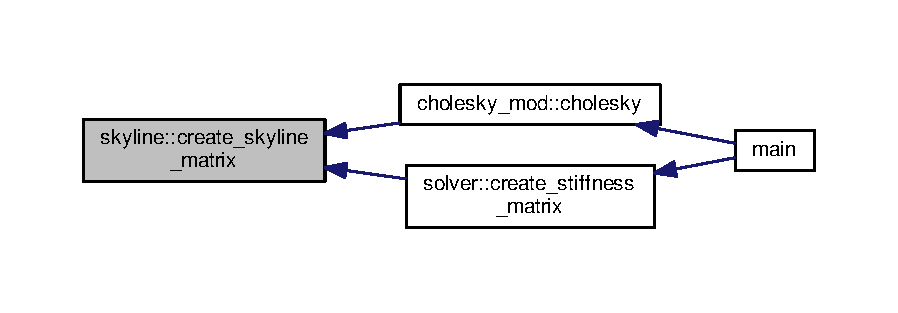
\includegraphics[width=350pt]{namespaceskyline_a5fe1d351df2e3a07f96028d1d2a892a8_icgraph}
\end{center}
\end{figure}
\mbox{\Hypertarget{namespaceskyline_a86a4fe28bc106ef42d25cf7596c108bf}\label{namespaceskyline_a86a4fe28bc106ef42d25cf7596c108bf}} 
\index{skyline@{skyline}!create\+\_\+skyline\+\_\+matrix\+\_\+from\+\_\+file@{create\+\_\+skyline\+\_\+matrix\+\_\+from\+\_\+file}}
\index{create\+\_\+skyline\+\_\+matrix\+\_\+from\+\_\+file@{create\+\_\+skyline\+\_\+matrix\+\_\+from\+\_\+file}!skyline@{skyline}}
\subsubsection{\texorpdfstring{create\+\_\+skyline\+\_\+matrix\+\_\+from\+\_\+file()}{create\_skyline\_matrix\_from\_file()}}
{\footnotesize\ttfamily type (\hyperlink{structskyline_1_1skyline__matrix}{skyline\+\_\+matrix}) function skyline\+::create\+\_\+skyline\+\_\+matrix\+\_\+from\+\_\+file (\begin{DoxyParamCaption}\item[{character(len=$\ast$), intent(in)}]{filename }\end{DoxyParamCaption})}



Créé une matrice S\+K\+Y\+L\+I\+NE depuis les données contenus dans un fichier. 


\begin{DoxyParams}{Parameters}
{\em filename} & Nom du fichier \\
\hline
\end{DoxyParams}
\begin{DoxyReturn}{Returns}
Matrice S\+K\+Y\+L\+I\+NE 
\end{DoxyReturn}
\mbox{\Hypertarget{namespaceskyline_a428818245223fbf6e3a5a2264f8f1a65}\label{namespaceskyline_a428818245223fbf6e3a5a2264f8f1a65}} 
\index{skyline@{skyline}!display@{display}}
\index{display@{display}!skyline@{skyline}}
\subsubsection{\texorpdfstring{display()}{display()}}
{\footnotesize\ttfamily subroutine skyline\+::display (\begin{DoxyParamCaption}\item[{class(\hyperlink{structskyline_1_1skyline__matrix}{skyline\+\_\+matrix}), intent(in)}]{M }\end{DoxyParamCaption})}



Affiche une matrice S\+K\+Y\+L\+I\+NE. 


\begin{DoxyParams}{Parameters}
{\em M} & Matrice S\+K\+Y\+L\+I\+NE \\
\hline
\end{DoxyParams}
Here is the call graph for this function\+:\nopagebreak
\begin{figure}[H]
\begin{center}
\leavevmode
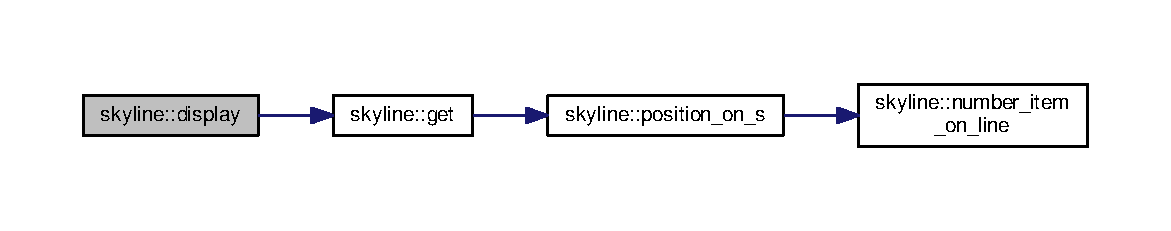
\includegraphics[width=350pt]{namespaceskyline_a428818245223fbf6e3a5a2264f8f1a65_cgraph}
\end{center}
\end{figure}
\mbox{\Hypertarget{namespaceskyline_aedb0d55aecd5f4cae4dc3593a5e89f0f}\label{namespaceskyline_aedb0d55aecd5f4cae4dc3593a5e89f0f}} 
\index{skyline@{skyline}!display\+\_\+debug@{display\+\_\+debug}}
\index{display\+\_\+debug@{display\+\_\+debug}!skyline@{skyline}}
\subsubsection{\texorpdfstring{display\+\_\+debug()}{display\_debug()}}
{\footnotesize\ttfamily subroutine skyline\+::display\+\_\+debug (\begin{DoxyParamCaption}\item[{class(\hyperlink{structskyline_1_1skyline__matrix}{skyline\+\_\+matrix}), intent(in)}]{M }\end{DoxyParamCaption})}



Affiche des informations de debuguage d\textquotesingle{}une matrice S\+K\+Y\+L\+I\+NE. 


\begin{DoxyParams}{Parameters}
{\em M} & Matrice S\+K\+Y\+L\+I\+NE \\
\hline
\end{DoxyParams}
\mbox{\Hypertarget{namespaceskyline_a583c70b26e3bcb37ecb679f5c11ec2f4}\label{namespaceskyline_a583c70b26e3bcb37ecb679f5c11ec2f4}} 
\index{skyline@{skyline}!free\+\_\+skyline\+\_\+matrix@{free\+\_\+skyline\+\_\+matrix}}
\index{free\+\_\+skyline\+\_\+matrix@{free\+\_\+skyline\+\_\+matrix}!skyline@{skyline}}
\subsubsection{\texorpdfstring{free\+\_\+skyline\+\_\+matrix()}{free\_skyline\_matrix()}}
{\footnotesize\ttfamily subroutine skyline\+::free\+\_\+skyline\+\_\+matrix (\begin{DoxyParamCaption}\item[{type(\hyperlink{structskyline_1_1skyline__matrix}{skyline\+\_\+matrix})}]{M }\end{DoxyParamCaption})}



Supprime les allocations mémoires d\textquotesingle{}une matrice S\+K\+Y\+L\+I\+NE. 


\begin{DoxyParams}{Parameters}
{\em M} & Matrice S\+K\+Y\+L\+I\+NE \\
\hline
\end{DoxyParams}
Here is the caller graph for this function\+:\nopagebreak
\begin{figure}[H]
\begin{center}
\leavevmode
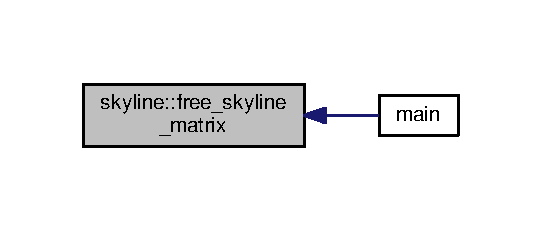
\includegraphics[width=260pt]{namespaceskyline_a583c70b26e3bcb37ecb679f5c11ec2f4_icgraph}
\end{center}
\end{figure}
\mbox{\Hypertarget{namespaceskyline_a28077ec6714b830771f90da1b674b0ce}\label{namespaceskyline_a28077ec6714b830771f90da1b674b0ce}} 
\index{skyline@{skyline}!get@{get}}
\index{get@{get}!skyline@{skyline}}
\subsubsection{\texorpdfstring{get()}{get()}}
{\footnotesize\ttfamily real function skyline\+::get (\begin{DoxyParamCaption}\item[{class(\hyperlink{structskyline_1_1skyline__matrix}{skyline\+\_\+matrix}), intent(in)}]{M,  }\item[{integer, intent(in)}]{row,  }\item[{integer, intent(in)}]{col }\end{DoxyParamCaption})}



Accède aux éléments d\textquotesingle{}une matrice S\+K\+Y\+L\+I\+NE. 


\begin{DoxyParams}{Parameters}
{\em M} & Matrice S\+K\+Y\+L\+I\+NE \\
\hline
{\em row} & Ligne de l\textquotesingle{}élément \\
\hline
{\em col} & Colonne de l\textquotesingle{}élément \\
\hline
\end{DoxyParams}
\begin{DoxyReturn}{Returns}
Valeur de M(i,j) 
\end{DoxyReturn}
Here is the call graph for this function\+:\nopagebreak
\begin{figure}[H]
\begin{center}
\leavevmode
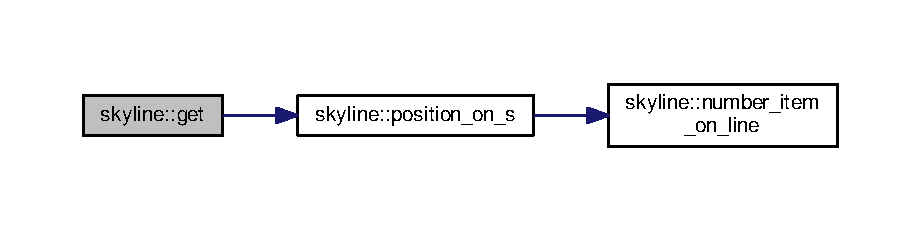
\includegraphics[width=350pt]{namespaceskyline_a28077ec6714b830771f90da1b674b0ce_cgraph}
\end{center}
\end{figure}
Here is the caller graph for this function\+:\nopagebreak
\begin{figure}[H]
\begin{center}
\leavevmode
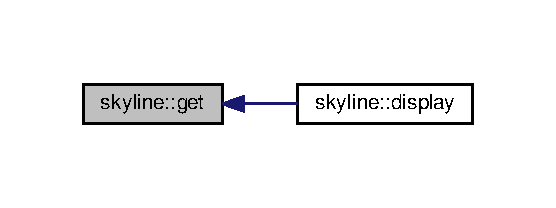
\includegraphics[width=267pt]{namespaceskyline_a28077ec6714b830771f90da1b674b0ce_icgraph}
\end{center}
\end{figure}
\mbox{\Hypertarget{namespaceskyline_a9f07218be321c12bea1d84f6b629e346}\label{namespaceskyline_a9f07218be321c12bea1d84f6b629e346}} 
\index{skyline@{skyline}!number\+\_\+item\+\_\+on\+\_\+line@{number\+\_\+item\+\_\+on\+\_\+line}}
\index{number\+\_\+item\+\_\+on\+\_\+line@{number\+\_\+item\+\_\+on\+\_\+line}!skyline@{skyline}}
\subsubsection{\texorpdfstring{number\+\_\+item\+\_\+on\+\_\+line()}{number\_item\_on\_line()}}
{\footnotesize\ttfamily integer function skyline\+::number\+\_\+item\+\_\+on\+\_\+line (\begin{DoxyParamCaption}\item[{class(\hyperlink{structskyline_1_1skyline__matrix}{skyline\+\_\+matrix}), intent(in)}]{M,  }\item[{integer, intent(in)}]{row }\end{DoxyParamCaption})}



Calcule le nombre d\textquotesingle{}élément stocké sur une ligne. 


\begin{DoxyParams}{Parameters}
{\em M} & Matrice S\+K\+Y\+L\+I\+NE \\
\hline
{\em row} & Indice de ligne \\
\hline
\end{DoxyParams}
\begin{DoxyReturn}{Returns}
Nombre d\textquotesingle{}élément stocké sur une ligne 
\end{DoxyReturn}
Here is the caller graph for this function\+:\nopagebreak
\begin{figure}[H]
\begin{center}
\leavevmode
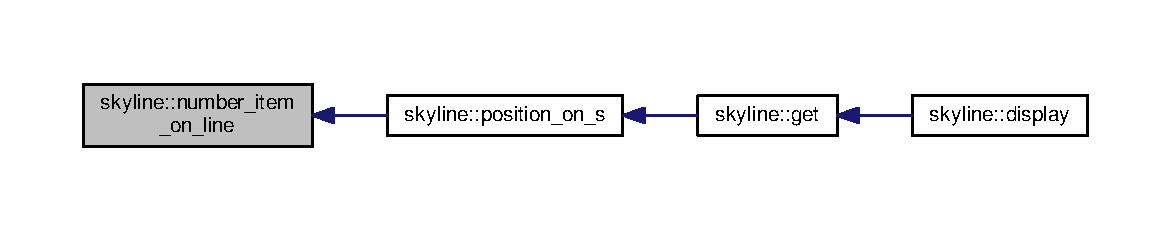
\includegraphics[width=350pt]{namespaceskyline_a9f07218be321c12bea1d84f6b629e346_icgraph}
\end{center}
\end{figure}
\mbox{\Hypertarget{namespaceskyline_a25b1e027d99abb67ab844d7b657a5843}\label{namespaceskyline_a25b1e027d99abb67ab844d7b657a5843}} 
\index{skyline@{skyline}!position\+\_\+on\+\_\+s@{position\+\_\+on\+\_\+s}}
\index{position\+\_\+on\+\_\+s@{position\+\_\+on\+\_\+s}!skyline@{skyline}}
\subsubsection{\texorpdfstring{position\+\_\+on\+\_\+s()}{position\_on\_s()}}
{\footnotesize\ttfamily integer function skyline\+::position\+\_\+on\+\_\+s (\begin{DoxyParamCaption}\item[{class(\hyperlink{structskyline_1_1skyline__matrix}{skyline\+\_\+matrix}), intent(in)}]{M,  }\item[{integer, intent(in)}]{row,  }\item[{integer, intent(in)}]{col }\end{DoxyParamCaption})}



Calcule la position d\textquotesingle{}un élément dans le tableau stockant les données. 


\begin{DoxyParams}{Parameters}
{\em M} & Matrice S\+K\+Y\+L\+I\+NE \\
\hline
{\em row} & Ligne de l\textquotesingle{}élément \\
\hline
{\em col} & Colonne de l\textquotesingle{}élément \\
\hline
\end{DoxyParams}
\begin{DoxyReturn}{Returns}
Indice de l\textquotesingle{}élément dans le tableau de donnée 
\end{DoxyReturn}
Here is the call graph for this function\+:\nopagebreak
\begin{figure}[H]
\begin{center}
\leavevmode
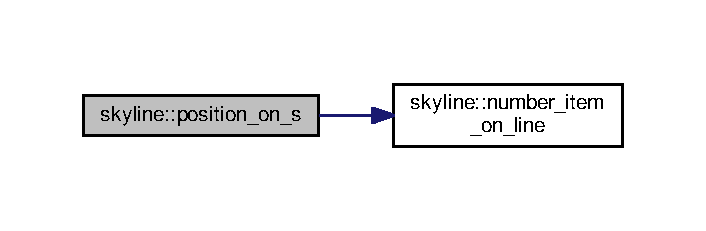
\includegraphics[width=339pt]{namespaceskyline_a25b1e027d99abb67ab844d7b657a5843_cgraph}
\end{center}
\end{figure}
Here is the caller graph for this function\+:\nopagebreak
\begin{figure}[H]
\begin{center}
\leavevmode
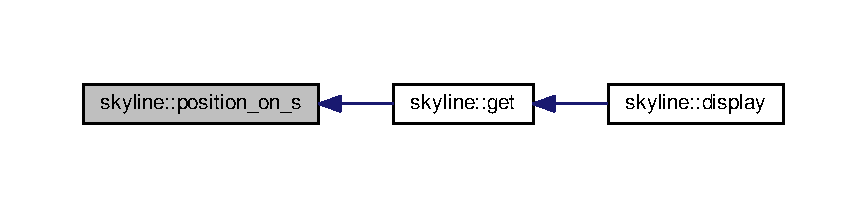
\includegraphics[width=350pt]{namespaceskyline_a25b1e027d99abb67ab844d7b657a5843_icgraph}
\end{center}
\end{figure}
\mbox{\Hypertarget{namespaceskyline_ae156a973c4a30bd2740af6ef2fdfa1d9}\label{namespaceskyline_ae156a973c4a30bd2740af6ef2fdfa1d9}} 
\index{skyline@{skyline}!prod\+\_\+mat\+\_\+vec@{prod\+\_\+mat\+\_\+vec}}
\index{prod\+\_\+mat\+\_\+vec@{prod\+\_\+mat\+\_\+vec}!skyline@{skyline}}
\subsubsection{\texorpdfstring{prod\+\_\+mat\+\_\+vec()}{prod\_mat\_vec()}}
{\footnotesize\ttfamily real function, dimension(\+:), allocatable skyline\+::prod\+\_\+mat\+\_\+vec (\begin{DoxyParamCaption}\item[{class(\hyperlink{structskyline_1_1skyline__matrix}{skyline\+\_\+matrix})}]{M,  }\item[{real, dimension(\+:), allocatable}]{X }\end{DoxyParamCaption})}



Calcule Le produit entre une matrice et un vecteur. 


\begin{DoxyParams}{Parameters}
{\em M} & Matrice S\+K\+Y\+L\+I\+NE \\
\hline
{\em X} & Vecteur \\
\hline
\end{DoxyParams}
\begin{DoxyReturn}{Returns}
Vecteur = M$\ast$X 
\end{DoxyReturn}
\mbox{\Hypertarget{namespaceskyline_a3377a8391ad2d61659689fc8c4130bdc}\label{namespaceskyline_a3377a8391ad2d61659689fc8c4130bdc}} 
\index{skyline@{skyline}!write\+\_\+skyline\+\_\+matrix\+\_\+to\+\_\+file@{write\+\_\+skyline\+\_\+matrix\+\_\+to\+\_\+file}}
\index{write\+\_\+skyline\+\_\+matrix\+\_\+to\+\_\+file@{write\+\_\+skyline\+\_\+matrix\+\_\+to\+\_\+file}!skyline@{skyline}}
\subsubsection{\texorpdfstring{write\+\_\+skyline\+\_\+matrix\+\_\+to\+\_\+file()}{write\_skyline\_matrix\_to\_file()}}
{\footnotesize\ttfamily subroutine skyline\+::write\+\_\+skyline\+\_\+matrix\+\_\+to\+\_\+file (\begin{DoxyParamCaption}\item[{type (\hyperlink{structskyline_1_1skyline__matrix}{skyline\+\_\+matrix})}]{M,  }\item[{character(len=$\ast$), intent(in)}]{filename }\end{DoxyParamCaption})}



Sauvegarde une matrice S\+K\+Y\+L\+I\+NE dans un fichier. 


\begin{DoxyParams}{Parameters}
{\em M} & Matrice à sauvegarder \\
\hline
{\em filename} & Nom du fichier \\
\hline
\end{DoxyParams}

\hypertarget{namespacesolver}{}\section{solver Module Reference}
\label{namespacesolver}\index{solver@{solver}}


Ce module permet de résoudre un problème d\textquotesingle{}éléments fini.  


\subsection*{Functions/\+Subroutines}
\begin{DoxyCompactItemize}
\item 
real function \hyperlink{namespacesolver_ab0081bb7880652eb26e65994f13fcb54}{a} (x)
\begin{DoxyCompactList}\small\item\em Fonction A(x) du problème donné \end{DoxyCompactList}\item 
real function \hyperlink{namespacesolver_a6f4d43c88c7c8ebdea64bd45e002af05}{f} (x)
\begin{DoxyCompactList}\small\item\em Fonction F(x) du problème donné \end{DoxyCompactList}\item 
logical function \hyperlink{namespacesolver_a2380e35eaa6fcef040f90bb5b23baa6a}{is\+\_\+in\+\_\+interval} (x, xmin, xmax)
\begin{DoxyCompactList}\small\item\em Calcule si une valeur est dans un intervalle donné \end{DoxyCompactList}\item 
real function \hyperlink{namespacesolver_a3323b7ad7f72685a465733177c82e8cc}{phi} (i, x, h, Xdiscret)
\begin{DoxyCompactList}\small\item\em Fonction de base. \end{DoxyCompactList}\item 
real function \hyperlink{namespacesolver_add1e5803b09e373fde46731960030e42}{phi\+\_\+der} (i, x, h, Xdiscret)
\begin{DoxyCompactList}\small\item\em Dérivée de la fonction de base. \end{DoxyCompactList}\item 
real function \hyperlink{namespacesolver_a5cdc774a6979796cb6b072b2fbb0e5af}{trapza} (binf, bsup, N)
\begin{DoxyCompactList}\small\item\em Calcul de l\textquotesingle{}intégrale du terme bilinéaire. \end{DoxyCompactList}\item 
real function \hyperlink{namespacesolver_adb6590794b23eaed708cd2e42adac550}{trapzf} (binf, bsup, N, ix, hx, Xdiscret)
\begin{DoxyCompactList}\small\item\em Calcul de l\textquotesingle{}intégrale du terme Linéaire. \end{DoxyCompactList}\item 
real function \hyperlink{namespacesolver_a99565d1c8ed5142211b78fe3ccca060b}{b} (i, j, h, Xdiscret, Nitg)
\begin{DoxyCompactList}\small\item\em Evaluation du terme bilinéaire. \end{DoxyCompactList}\item 
real function \hyperlink{namespacesolver_a327c990a10263590618db7a31c4edcc9}{l} (i, h, Xdiscret, Nitg, alpha1)
\begin{DoxyCompactList}\small\item\em Evaluation du terme Linéaire. \end{DoxyCompactList}\item 
type(skyline\+\_\+matrix) function \hyperlink{namespacesolver_aefd2f88bd66b9d9ccce170259a49c77d}{create\+\_\+stiffness\+\_\+matrix} (h, Xdiscret, Nitg)
\begin{DoxyCompactList}\small\item\em Calcul la matrice de rigidité \end{DoxyCompactList}\item 
real function, dimension(\+:), allocatable \hyperlink{namespacesolver_af45a5f246a818112e6a257335c2b829d}{create\+\_\+f\+\_\+matrix} (h, Xdiscret, Nitg, alpha1)
\begin{DoxyCompactList}\small\item\em Calcule du second membre. \end{DoxyCompactList}\item 
real function, dimension(\+:), allocatable \hyperlink{namespacesolver_ad8b8ef6c982475b3fb276f93660b750f}{solve\+\_\+trig\+\_\+down} (LT, BB)
\begin{DoxyCompactList}\small\item\em Résouds le système triangulaire inférieur. \end{DoxyCompactList}\item 
real function, dimension(\+:), allocatable \hyperlink{namespacesolver_a08b8f70c86d7bf39b32ce8fdcc872fd4}{solve\+\_\+trig\+\_\+up} (LT, BB)
\begin{DoxyCompactList}\small\item\em Résouds le système triangulaire supérieur. \end{DoxyCompactList}\item 
real function, dimension(\+:), allocatable \hyperlink{namespacesolver_af3691d2059a024a82bab7751a99e6006}{solve} (LT, BB)
\begin{DoxyCompactList}\small\item\em Résouds le problème $ LT*Y = BB$. \end{DoxyCompactList}\item 
subroutine \hyperlink{namespacesolver_a2456ddba19a0992671f59ac396d4c1f1}{export\+\_\+solution} (Xdiscret, U, filename)
\begin{DoxyCompactList}\small\item\em Enregistre un vecteur solution dans un fichier. \end{DoxyCompactList}\end{DoxyCompactItemize}


\subsection{Detailed Description}
Ce module permet de résoudre un problème d\textquotesingle{}éléments fini. 

\begin{DoxyAuthor}{Author}
Kara Abdelhadi, Mechineau Alexandre 
\end{DoxyAuthor}


\subsection{Function/\+Subroutine Documentation}
\mbox{\Hypertarget{namespacesolver_ab0081bb7880652eb26e65994f13fcb54}\label{namespacesolver_ab0081bb7880652eb26e65994f13fcb54}} 
\index{solver@{solver}!a@{a}}
\index{a@{a}!solver@{solver}}
\subsubsection{\texorpdfstring{a()}{a()}}
{\footnotesize\ttfamily real function solver\+::a (\begin{DoxyParamCaption}\item[{real}]{x }\end{DoxyParamCaption})}



Fonction A(x) du problème donné 


\begin{DoxyParams}{Parameters}
{\em x} & Réel \\
\hline
\end{DoxyParams}
\begin{DoxyReturn}{Returns}
A(x) 
\end{DoxyReturn}
Here is the caller graph for this function\+:\nopagebreak
\begin{figure}[H]
\begin{center}
\leavevmode
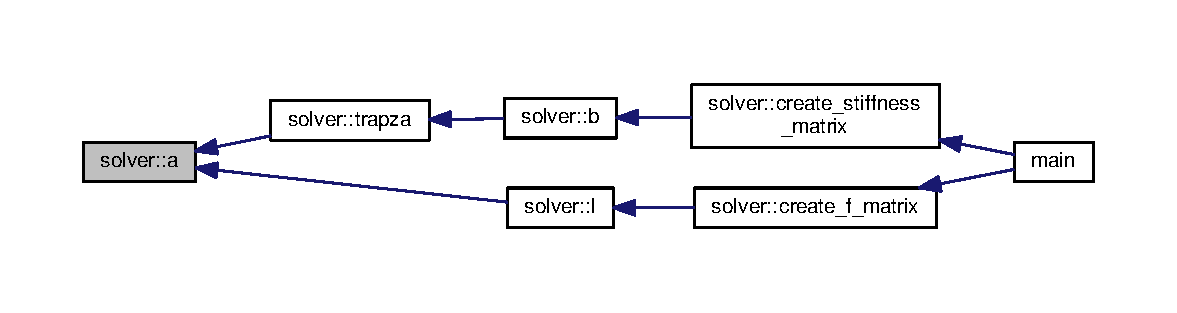
\includegraphics[width=350pt]{namespacesolver_ab0081bb7880652eb26e65994f13fcb54_icgraph}
\end{center}
\end{figure}
\mbox{\Hypertarget{namespacesolver_a99565d1c8ed5142211b78fe3ccca060b}\label{namespacesolver_a99565d1c8ed5142211b78fe3ccca060b}} 
\index{solver@{solver}!b@{b}}
\index{b@{b}!solver@{solver}}
\subsubsection{\texorpdfstring{b()}{b()}}
{\footnotesize\ttfamily real function solver\+::b (\begin{DoxyParamCaption}\item[{integer}]{i,  }\item[{integer}]{j,  }\item[{real}]{h,  }\item[{real, dimension(\+:), allocatable}]{Xdiscret,  }\item[{integer}]{Nitg }\end{DoxyParamCaption})}



Evaluation du terme bilinéaire. 


\begin{DoxyParams}{Parameters}
{\em i} & Indice Ligne \\
\hline
{\em j} & Indice colonne \\
\hline
{\em h} & Pas du maillage \\
\hline
{\em Xdiscret} & Maillage \\
\hline
{\em Nitg} & Précision intégration \\
\hline
\end{DoxyParams}
\begin{DoxyReturn}{Returns}

\end{DoxyReturn}
Here is the call graph for this function\+:\nopagebreak
\begin{figure}[H]
\begin{center}
\leavevmode
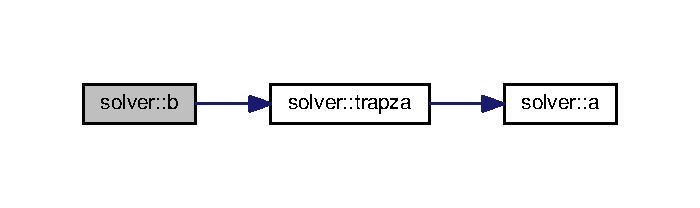
\includegraphics[width=336pt]{namespacesolver_a99565d1c8ed5142211b78fe3ccca060b_cgraph}
\end{center}
\end{figure}
Here is the caller graph for this function\+:\nopagebreak
\begin{figure}[H]
\begin{center}
\leavevmode
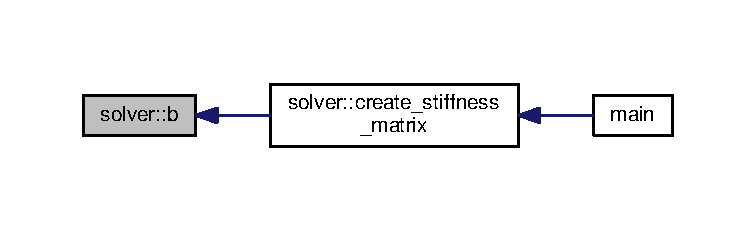
\includegraphics[width=350pt]{namespacesolver_a99565d1c8ed5142211b78fe3ccca060b_icgraph}
\end{center}
\end{figure}
\mbox{\Hypertarget{namespacesolver_af45a5f246a818112e6a257335c2b829d}\label{namespacesolver_af45a5f246a818112e6a257335c2b829d}} 
\index{solver@{solver}!create\+\_\+f\+\_\+matrix@{create\+\_\+f\+\_\+matrix}}
\index{create\+\_\+f\+\_\+matrix@{create\+\_\+f\+\_\+matrix}!solver@{solver}}
\subsubsection{\texorpdfstring{create\+\_\+f\+\_\+matrix()}{create\_f\_matrix()}}
{\footnotesize\ttfamily real function, dimension(\+:), allocatable solver\+::create\+\_\+f\+\_\+matrix (\begin{DoxyParamCaption}\item[{real}]{h,  }\item[{real, dimension(\+:), allocatable}]{Xdiscret,  }\item[{integer}]{Nitg,  }\item[{real}]{alpha1 }\end{DoxyParamCaption})}



Calcule du second membre. 


\begin{DoxyParams}{Parameters}
{\em h} & Pas du maillage \\
\hline
{\em Xdiscret} & Maillage \\
\hline
{\em Nitg} & Précision intégration \\
\hline
{\em alpha1} & Parametre du problème \\
\hline
\end{DoxyParams}
\begin{DoxyReturn}{Returns}
Matrice S\+K\+Y\+L\+I\+NE 
\end{DoxyReturn}
Here is the call graph for this function\+:\nopagebreak
\begin{figure}[H]
\begin{center}
\leavevmode
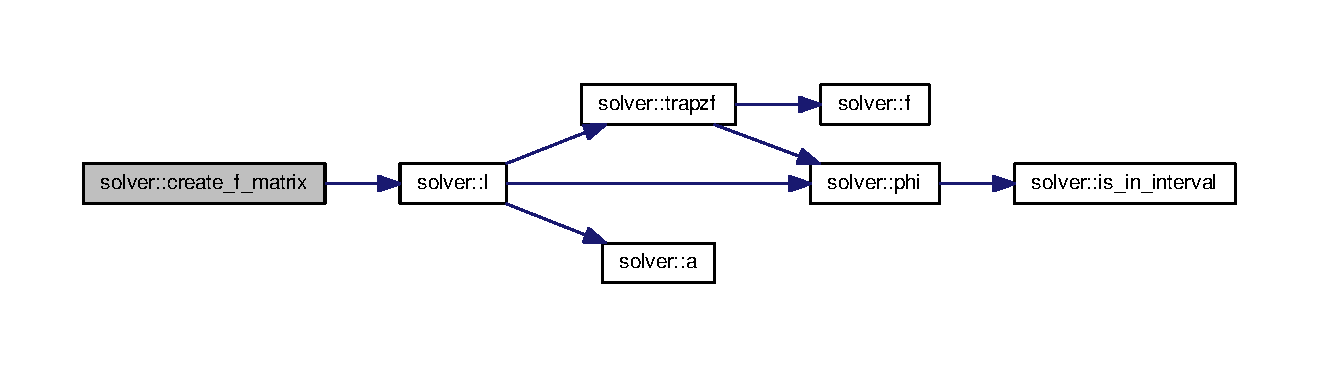
\includegraphics[width=350pt]{namespacesolver_af45a5f246a818112e6a257335c2b829d_cgraph}
\end{center}
\end{figure}
Here is the caller graph for this function\+:\nopagebreak
\begin{figure}[H]
\begin{center}
\leavevmode
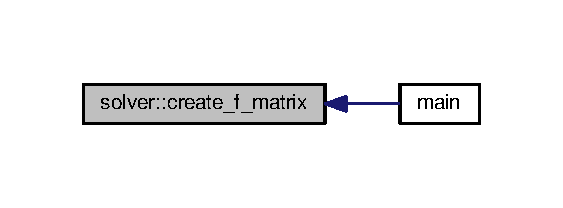
\includegraphics[width=270pt]{namespacesolver_af45a5f246a818112e6a257335c2b829d_icgraph}
\end{center}
\end{figure}
\mbox{\Hypertarget{namespacesolver_aefd2f88bd66b9d9ccce170259a49c77d}\label{namespacesolver_aefd2f88bd66b9d9ccce170259a49c77d}} 
\index{solver@{solver}!create\+\_\+stiffness\+\_\+matrix@{create\+\_\+stiffness\+\_\+matrix}}
\index{create\+\_\+stiffness\+\_\+matrix@{create\+\_\+stiffness\+\_\+matrix}!solver@{solver}}
\subsubsection{\texorpdfstring{create\+\_\+stiffness\+\_\+matrix()}{create\_stiffness\_matrix()}}
{\footnotesize\ttfamily type(skyline\+\_\+matrix) function solver\+::create\+\_\+stiffness\+\_\+matrix (\begin{DoxyParamCaption}\item[{real}]{h,  }\item[{real, dimension(\+:), allocatable}]{Xdiscret,  }\item[{integer}]{Nitg }\end{DoxyParamCaption})}



Calcul la matrice de rigidité 


\begin{DoxyParams}{Parameters}
{\em h} & Pas du maillage \\
\hline
{\em Xdiscret} & Maillage \\
\hline
{\em Nitg} & Précision intégration \\
\hline
\end{DoxyParams}
\begin{DoxyReturn}{Returns}
Matrice S\+K\+Y\+L\+I\+NE 
\end{DoxyReturn}
Here is the call graph for this function\+:\nopagebreak
\begin{figure}[H]
\begin{center}
\leavevmode
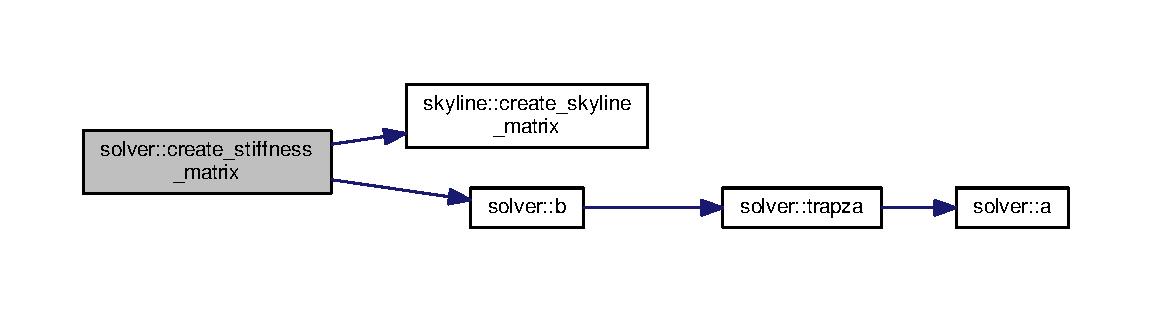
\includegraphics[width=350pt]{namespacesolver_aefd2f88bd66b9d9ccce170259a49c77d_cgraph}
\end{center}
\end{figure}
Here is the caller graph for this function\+:\nopagebreak
\begin{figure}[H]
\begin{center}
\leavevmode
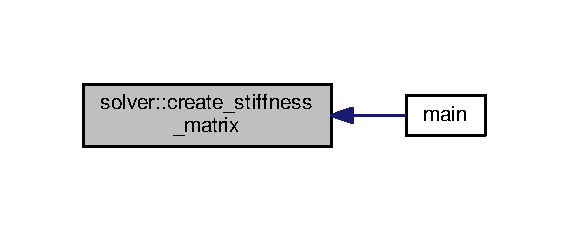
\includegraphics[width=273pt]{namespacesolver_aefd2f88bd66b9d9ccce170259a49c77d_icgraph}
\end{center}
\end{figure}
\mbox{\Hypertarget{namespacesolver_a2456ddba19a0992671f59ac396d4c1f1}\label{namespacesolver_a2456ddba19a0992671f59ac396d4c1f1}} 
\index{solver@{solver}!export\+\_\+solution@{export\+\_\+solution}}
\index{export\+\_\+solution@{export\+\_\+solution}!solver@{solver}}
\subsubsection{\texorpdfstring{export\+\_\+solution()}{export\_solution()}}
{\footnotesize\ttfamily subroutine solver\+::export\+\_\+solution (\begin{DoxyParamCaption}\item[{real, dimension(\+:), allocatable}]{Xdiscret,  }\item[{real, dimension(\+:), allocatable}]{U,  }\item[{character(len=$\ast$), intent(in)}]{filename }\end{DoxyParamCaption})}



Enregistre un vecteur solution dans un fichier. 


\begin{DoxyParams}{Parameters}
{\em Xdiscret} & Discrétisation espace \\
\hline
{\em U} & Vecteur solution \\
\hline
{\em filename} & Nom du fichier \\
\hline
\end{DoxyParams}
Here is the caller graph for this function\+:
\nopagebreak
\begin{figure}[H]
\begin{center}
\leavevmode
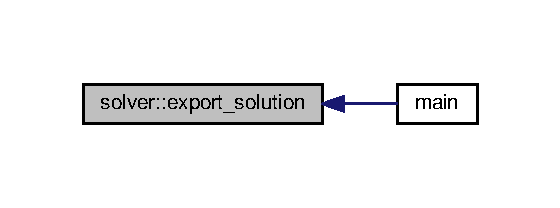
\includegraphics[width=269pt]{namespacesolver_a2456ddba19a0992671f59ac396d4c1f1_icgraph}
\end{center}
\end{figure}
\mbox{\Hypertarget{namespacesolver_a6f4d43c88c7c8ebdea64bd45e002af05}\label{namespacesolver_a6f4d43c88c7c8ebdea64bd45e002af05}} 
\index{solver@{solver}!f@{f}}
\index{f@{f}!solver@{solver}}
\subsubsection{\texorpdfstring{f()}{f()}}
{\footnotesize\ttfamily real function solver\+::f (\begin{DoxyParamCaption}\item[{real}]{x }\end{DoxyParamCaption})}



Fonction F(x) du problème donné 


\begin{DoxyParams}{Parameters}
{\em x} & Réel \\
\hline
\end{DoxyParams}
\begin{DoxyReturn}{Returns}
F(x) 
\end{DoxyReturn}
Here is the caller graph for this function\+:
\nopagebreak
\begin{figure}[H]
\begin{center}
\leavevmode
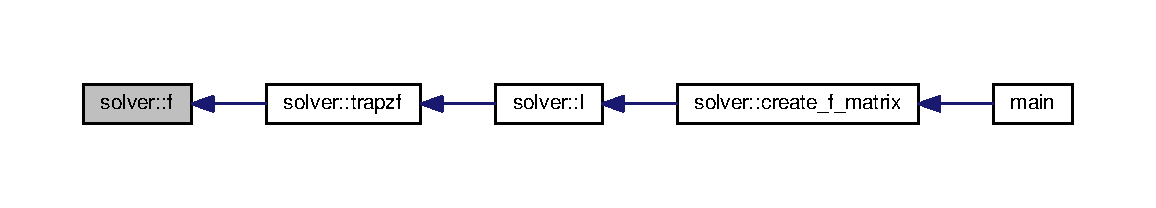
\includegraphics[width=350pt]{namespacesolver_a6f4d43c88c7c8ebdea64bd45e002af05_icgraph}
\end{center}
\end{figure}
\mbox{\Hypertarget{namespacesolver_a2380e35eaa6fcef040f90bb5b23baa6a}\label{namespacesolver_a2380e35eaa6fcef040f90bb5b23baa6a}} 
\index{solver@{solver}!is\+\_\+in\+\_\+interval@{is\+\_\+in\+\_\+interval}}
\index{is\+\_\+in\+\_\+interval@{is\+\_\+in\+\_\+interval}!solver@{solver}}
\subsubsection{\texorpdfstring{is\+\_\+in\+\_\+interval()}{is\_in\_interval()}}
{\footnotesize\ttfamily logical function solver\+::is\+\_\+in\+\_\+interval (\begin{DoxyParamCaption}\item[{real}]{x,  }\item[{real}]{xmin,  }\item[{real}]{xmax }\end{DoxyParamCaption})}



Calcule si une valeur est dans un intervalle donné 


\begin{DoxyParams}{Parameters}
{\em x} & Valeur \\
\hline
{\em xmin} & Borne inf de l\textquotesingle{}intervalle \\
\hline
{\em xmax} & Borne max de l\textquotesingle{}intervalle \\
\hline
\end{DoxyParams}
\begin{DoxyReturn}{Returns}
L\+O\+G\+I\+C\+AL 
\end{DoxyReturn}
Here is the caller graph for this function\+:
\nopagebreak
\begin{figure}[H]
\begin{center}
\leavevmode
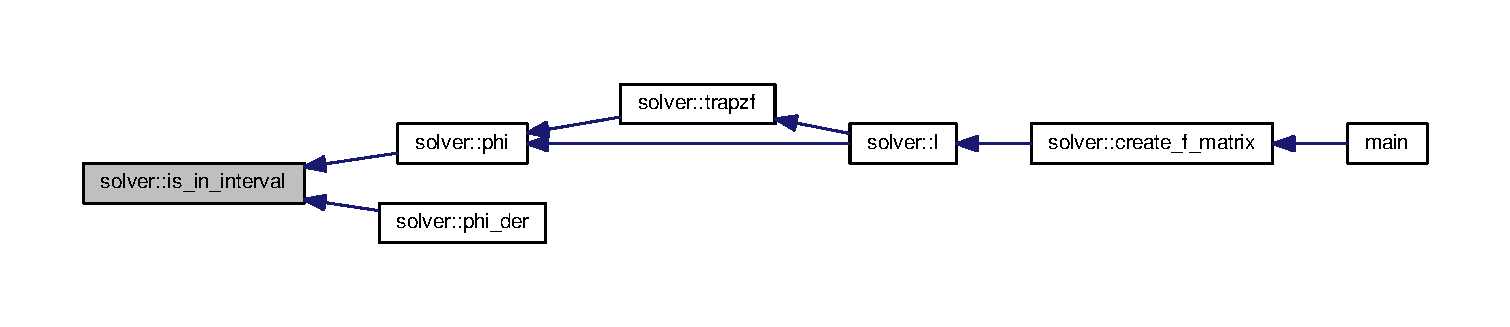
\includegraphics[width=350pt]{namespacesolver_a2380e35eaa6fcef040f90bb5b23baa6a_icgraph}
\end{center}
\end{figure}
\mbox{\Hypertarget{namespacesolver_a327c990a10263590618db7a31c4edcc9}\label{namespacesolver_a327c990a10263590618db7a31c4edcc9}} 
\index{solver@{solver}!l@{l}}
\index{l@{l}!solver@{solver}}
\subsubsection{\texorpdfstring{l()}{l()}}
{\footnotesize\ttfamily real function solver\+::l (\begin{DoxyParamCaption}\item[{integer}]{i,  }\item[{real}]{h,  }\item[{real, dimension(\+:), allocatable}]{Xdiscret,  }\item[{integer}]{Nitg,  }\item[{real}]{alpha1 }\end{DoxyParamCaption})}



Evaluation du terme Linéaire. 


\begin{DoxyParams}{Parameters}
{\em i} & Indice ligne \\
\hline
{\em h} & Pas du maillage \\
\hline
{\em Xdiscret} & Maillage \\
\hline
{\em Nitg} & Précision intégration \\
\hline
{\em alpha1} & Parametre du problème \\
\hline
\end{DoxyParams}
\begin{DoxyReturn}{Returns}

\end{DoxyReturn}
Here is the call graph for this function\+:
\nopagebreak
\begin{figure}[H]
\begin{center}
\leavevmode
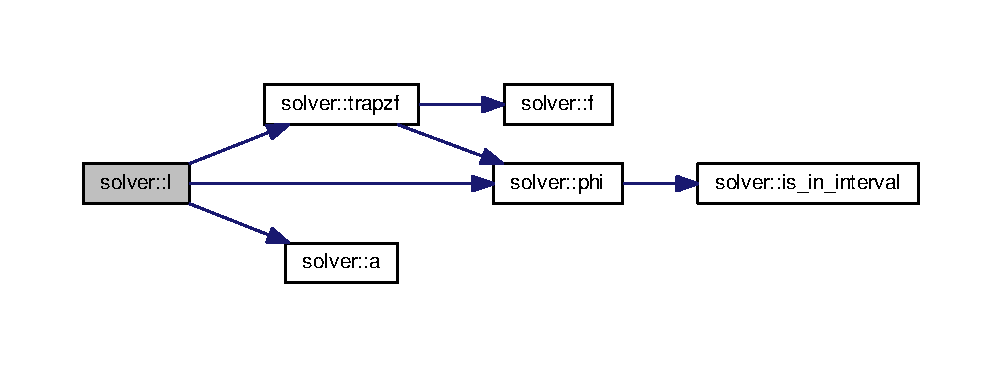
\includegraphics[width=350pt]{namespacesolver_a327c990a10263590618db7a31c4edcc9_cgraph}
\end{center}
\end{figure}
Here is the caller graph for this function\+:
\nopagebreak
\begin{figure}[H]
\begin{center}
\leavevmode
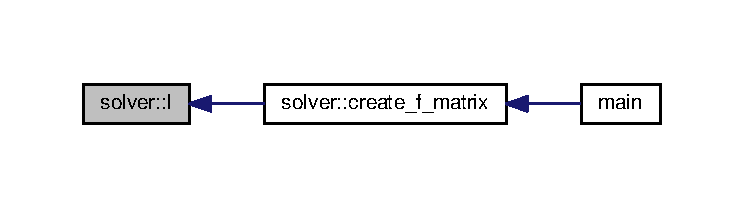
\includegraphics[width=350pt]{namespacesolver_a327c990a10263590618db7a31c4edcc9_icgraph}
\end{center}
\end{figure}
\mbox{\Hypertarget{namespacesolver_a3323b7ad7f72685a465733177c82e8cc}\label{namespacesolver_a3323b7ad7f72685a465733177c82e8cc}} 
\index{solver@{solver}!phi@{phi}}
\index{phi@{phi}!solver@{solver}}
\subsubsection{\texorpdfstring{phi()}{phi()}}
{\footnotesize\ttfamily real function solver\+::phi (\begin{DoxyParamCaption}\item[{integer}]{i,  }\item[{real}]{x,  }\item[{real}]{h,  }\item[{real, dimension(\+:), allocatable}]{Xdiscret }\end{DoxyParamCaption})}



Fonction de base. 


\begin{DoxyParams}{Parameters}
{\em i} & Indice de la fonction \\
\hline
{\em x} & Valeur d\textquotesingle{}évaluation \\
\hline
{\em h} & Pas de discrétisation \\
\hline
{\em Xdiscret} & Maillage \\
\hline
\end{DoxyParams}
\begin{DoxyReturn}{Returns}
Evaluation de $PHI_i$ en x 
\end{DoxyReturn}
Here is the call graph for this function\+:
\nopagebreak
\begin{figure}[H]
\begin{center}
\leavevmode
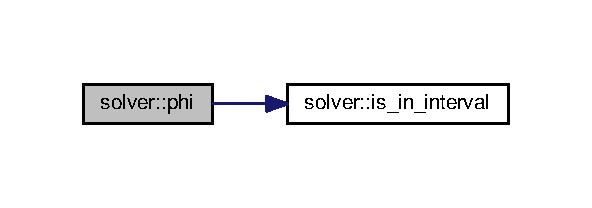
\includegraphics[width=284pt]{namespacesolver_a3323b7ad7f72685a465733177c82e8cc_cgraph}
\end{center}
\end{figure}
Here is the caller graph for this function\+:
\nopagebreak
\begin{figure}[H]
\begin{center}
\leavevmode
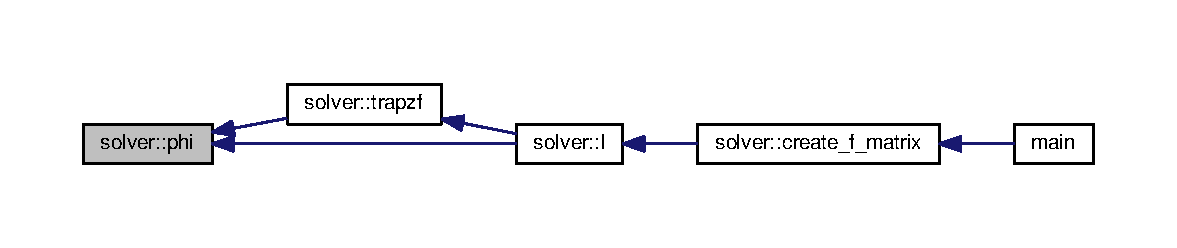
\includegraphics[width=350pt]{namespacesolver_a3323b7ad7f72685a465733177c82e8cc_icgraph}
\end{center}
\end{figure}
\mbox{\Hypertarget{namespacesolver_add1e5803b09e373fde46731960030e42}\label{namespacesolver_add1e5803b09e373fde46731960030e42}} 
\index{solver@{solver}!phi\+\_\+der@{phi\+\_\+der}}
\index{phi\+\_\+der@{phi\+\_\+der}!solver@{solver}}
\subsubsection{\texorpdfstring{phi\+\_\+der()}{phi\_der()}}
{\footnotesize\ttfamily real function solver\+::phi\+\_\+der (\begin{DoxyParamCaption}\item[{integer}]{i,  }\item[{real}]{x,  }\item[{real}]{h,  }\item[{real, dimension(\+:), allocatable}]{Xdiscret }\end{DoxyParamCaption})}



Dérivée de la fonction de base. 


\begin{DoxyParams}{Parameters}
{\em i} & Indice de la fonction \\
\hline
{\em x} & Valeur d\textquotesingle{}évaluation \\
\hline
{\em h} & Pas de discrétisation \\
\hline
{\em Xdiscret} & Maillage \\
\hline
\end{DoxyParams}
\begin{DoxyReturn}{Returns}
Evaluation de la dérivée de $PHI_i$ en x 
\end{DoxyReturn}
Here is the call graph for this function\+:
\nopagebreak
\begin{figure}[H]
\begin{center}
\leavevmode
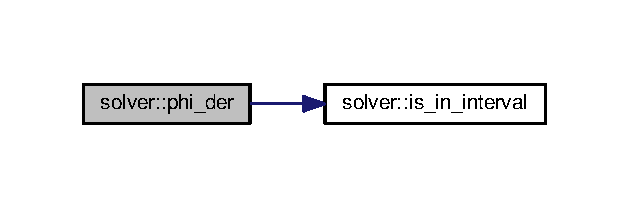
\includegraphics[width=302pt]{namespacesolver_add1e5803b09e373fde46731960030e42_cgraph}
\end{center}
\end{figure}
\mbox{\Hypertarget{namespacesolver_af3691d2059a024a82bab7751a99e6006}\label{namespacesolver_af3691d2059a024a82bab7751a99e6006}} 
\index{solver@{solver}!solve@{solve}}
\index{solve@{solve}!solver@{solver}}
\subsubsection{\texorpdfstring{solve()}{solve()}}
{\footnotesize\ttfamily real function, dimension(\+:), allocatable solver\+::solve (\begin{DoxyParamCaption}\item[{type(skyline\+\_\+matrix)}]{LT,  }\item[{real, dimension(\+:), allocatable}]{BB }\end{DoxyParamCaption})}



Résouds le problème $ LT*Y = BB$. 


\begin{DoxyParams}{Parameters}
{\em LT} & Matrice S\+K\+Y\+L\+I\+NE \\
\hline
{\em BB} & second membre \\
\hline
\end{DoxyParams}
\begin{DoxyReturn}{Returns}
Vecteur Solution 
\end{DoxyReturn}
Here is the call graph for this function\+:
\nopagebreak
\begin{figure}[H]
\begin{center}
\leavevmode
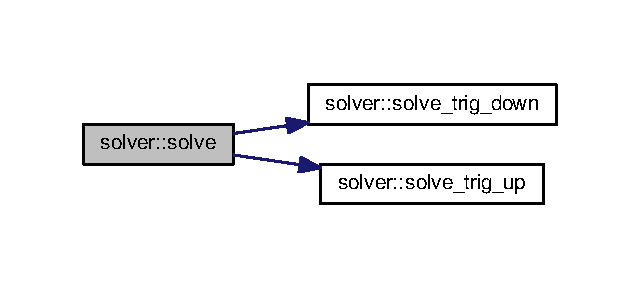
\includegraphics[width=307pt]{namespacesolver_af3691d2059a024a82bab7751a99e6006_cgraph}
\end{center}
\end{figure}
Here is the caller graph for this function\+:
\nopagebreak
\begin{figure}[H]
\begin{center}
\leavevmode
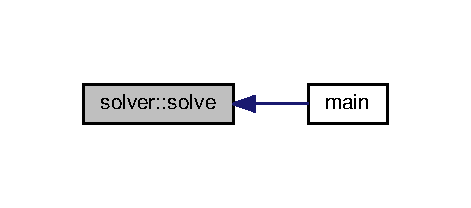
\includegraphics[width=226pt]{namespacesolver_af3691d2059a024a82bab7751a99e6006_icgraph}
\end{center}
\end{figure}
\mbox{\Hypertarget{namespacesolver_ad8b8ef6c982475b3fb276f93660b750f}\label{namespacesolver_ad8b8ef6c982475b3fb276f93660b750f}} 
\index{solver@{solver}!solve\+\_\+trig\+\_\+down@{solve\+\_\+trig\+\_\+down}}
\index{solve\+\_\+trig\+\_\+down@{solve\+\_\+trig\+\_\+down}!solver@{solver}}
\subsubsection{\texorpdfstring{solve\+\_\+trig\+\_\+down()}{solve\_trig\_down()}}
{\footnotesize\ttfamily real function, dimension(\+:), allocatable solver\+::solve\+\_\+trig\+\_\+down (\begin{DoxyParamCaption}\item[{type(skyline\+\_\+matrix)}]{LT,  }\item[{real, dimension(\+:), allocatable}]{BB }\end{DoxyParamCaption})}



Résouds le système triangulaire inférieur. 


\begin{DoxyParams}{Parameters}
{\em LT} & Matrice S\+K\+Y\+L\+I\+NE \\
\hline
{\em BB} & second membre \\
\hline
\end{DoxyParams}
\begin{DoxyReturn}{Returns}
Vecteur Solution 
\end{DoxyReturn}
Here is the caller graph for this function\+:
\nopagebreak
\begin{figure}[H]
\begin{center}
\leavevmode
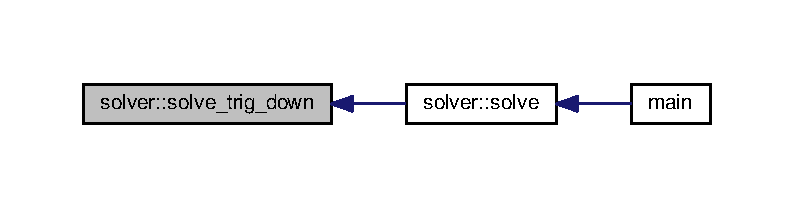
\includegraphics[width=350pt]{namespacesolver_ad8b8ef6c982475b3fb276f93660b750f_icgraph}
\end{center}
\end{figure}
\mbox{\Hypertarget{namespacesolver_a08b8f70c86d7bf39b32ce8fdcc872fd4}\label{namespacesolver_a08b8f70c86d7bf39b32ce8fdcc872fd4}} 
\index{solver@{solver}!solve\+\_\+trig\+\_\+up@{solve\+\_\+trig\+\_\+up}}
\index{solve\+\_\+trig\+\_\+up@{solve\+\_\+trig\+\_\+up}!solver@{solver}}
\subsubsection{\texorpdfstring{solve\+\_\+trig\+\_\+up()}{solve\_trig\_up()}}
{\footnotesize\ttfamily real function, dimension(\+:), allocatable solver\+::solve\+\_\+trig\+\_\+up (\begin{DoxyParamCaption}\item[{type(skyline\+\_\+matrix)}]{LT,  }\item[{real, dimension(\+:), allocatable}]{BB }\end{DoxyParamCaption})}



Résouds le système triangulaire supérieur. 


\begin{DoxyParams}{Parameters}
{\em LT} & Matrice S\+K\+Y\+L\+I\+NE \\
\hline
{\em BB} & second membre \\
\hline
\end{DoxyParams}
\begin{DoxyReturn}{Returns}
Vecteur Solution 
\end{DoxyReturn}
Here is the caller graph for this function\+:
\nopagebreak
\begin{figure}[H]
\begin{center}
\leavevmode
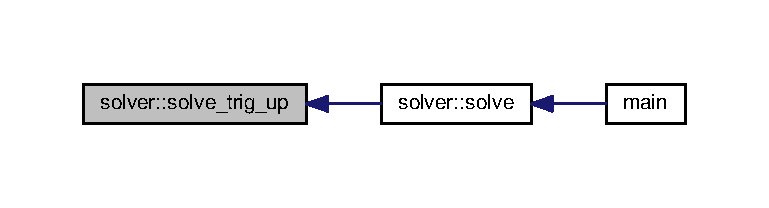
\includegraphics[width=350pt]{namespacesolver_a08b8f70c86d7bf39b32ce8fdcc872fd4_icgraph}
\end{center}
\end{figure}
\mbox{\Hypertarget{namespacesolver_a5cdc774a6979796cb6b072b2fbb0e5af}\label{namespacesolver_a5cdc774a6979796cb6b072b2fbb0e5af}} 
\index{solver@{solver}!trapza@{trapza}}
\index{trapza@{trapza}!solver@{solver}}
\subsubsection{\texorpdfstring{trapza()}{trapza()}}
{\footnotesize\ttfamily real function solver\+::trapza (\begin{DoxyParamCaption}\item[{real}]{binf,  }\item[{real}]{bsup,  }\item[{integer}]{N }\end{DoxyParamCaption})}



Calcul de l\textquotesingle{}intégrale du terme bilinéaire. 


\begin{DoxyParams}{Parameters}
{\em binf} & Borne inf \\
\hline
{\em bsup} & Borne sup \\
\hline
{\em N} & Précision de l\textquotesingle{}intégrale \\
\hline
\end{DoxyParams}
\begin{DoxyReturn}{Returns}
Valeur de l\textquotesingle{}intégrale 
\end{DoxyReturn}
Here is the call graph for this function\+:
\nopagebreak
\begin{figure}[H]
\begin{center}
\leavevmode
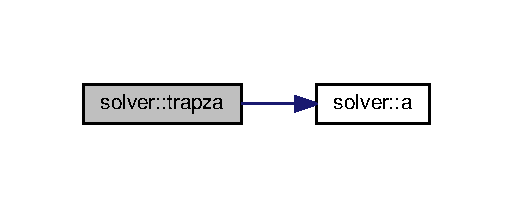
\includegraphics[width=246pt]{namespacesolver_a5cdc774a6979796cb6b072b2fbb0e5af_cgraph}
\end{center}
\end{figure}
Here is the caller graph for this function\+:
\nopagebreak
\begin{figure}[H]
\begin{center}
\leavevmode
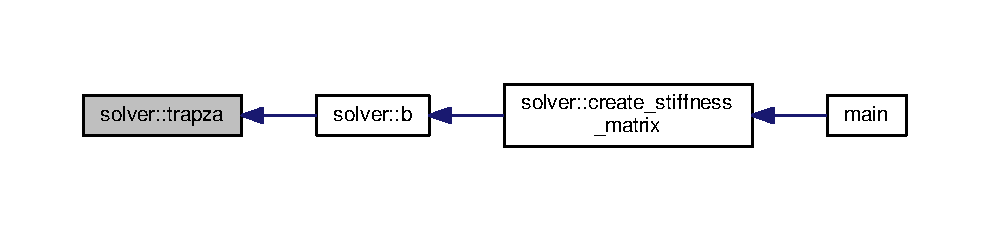
\includegraphics[width=350pt]{namespacesolver_a5cdc774a6979796cb6b072b2fbb0e5af_icgraph}
\end{center}
\end{figure}
\mbox{\Hypertarget{namespacesolver_adb6590794b23eaed708cd2e42adac550}\label{namespacesolver_adb6590794b23eaed708cd2e42adac550}} 
\index{solver@{solver}!trapzf@{trapzf}}
\index{trapzf@{trapzf}!solver@{solver}}
\subsubsection{\texorpdfstring{trapzf()}{trapzf()}}
{\footnotesize\ttfamily real function solver\+::trapzf (\begin{DoxyParamCaption}\item[{real}]{binf,  }\item[{real}]{bsup,  }\item[{integer}]{N,  }\item[{integer}]{ix,  }\item[{real}]{hx,  }\item[{real, dimension(\+:), allocatable}]{Xdiscret }\end{DoxyParamCaption})}



Calcul de l\textquotesingle{}intégrale du terme Linéaire. 


\begin{DoxyParams}{Parameters}
{\em binf} & Borne inf \\
\hline
{\em bsup} & Borne sup \\
\hline
{\em N} & Précision de l\textquotesingle{}intégrale \\
\hline
{\em ix} & Indice de la fonction P\+HI \\
\hline
{\em hx} & Pas du maillage \\
\hline
\end{DoxyParams}
\begin{DoxyReturn}{Returns}
Valeur de l\textquotesingle{}intégrale 
\end{DoxyReturn}
Here is the call graph for this function\+:
\nopagebreak
\begin{figure}[H]
\begin{center}
\leavevmode
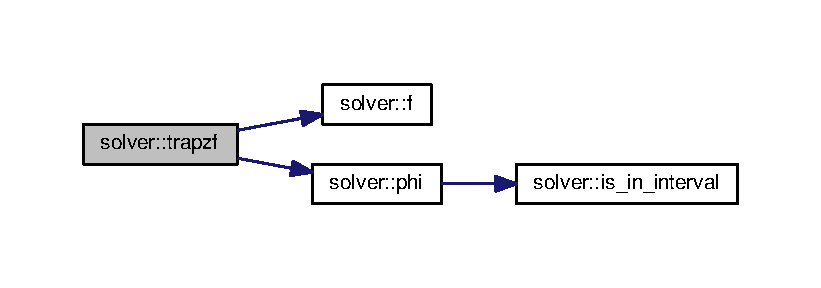
\includegraphics[width=350pt]{namespacesolver_adb6590794b23eaed708cd2e42adac550_cgraph}
\end{center}
\end{figure}
Here is the caller graph for this function\+:
\nopagebreak
\begin{figure}[H]
\begin{center}
\leavevmode
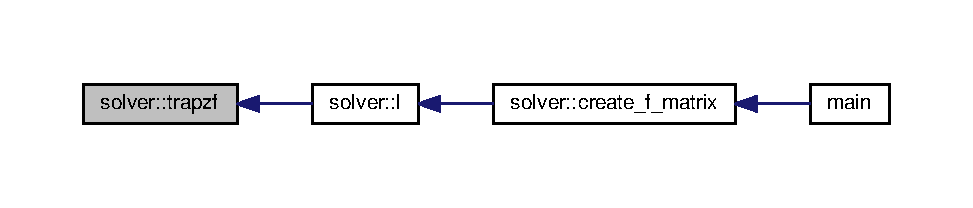
\includegraphics[width=350pt]{namespacesolver_adb6590794b23eaed708cd2e42adac550_icgraph}
\end{center}
\end{figure}

\chapter{Documentation du type de données}
\hypertarget{structskyline_1_1skyline__matrix}{}\section{skyline\+:\+:skyline\+\_\+matrix Type Reference}
\label{structskyline_1_1skyline__matrix}\index{skyline\+::skyline\+\_\+matrix@{skyline\+::skyline\+\_\+matrix}}
\subsection*{Public Member Functions}
\begin{DoxyCompactItemize}
\item 
P\+R\+O\+C\+E\+D\+U\+RE \hyperlink{structskyline_1_1skyline__matrix_a3b8d47decbf713171eb82625a51fbcd1}{get}
\item 
\hyperlink{structskyline_1_1skyline__matrix_ab03e03935f5904ed8f75d303c0bd291a}{display}
\item 
\hyperlink{structskyline_1_1skyline__matrix_ae32226cd0b3b93e3cb1ec3757642eb5e}{prod\+\_\+mat\+\_\+vec}
\item 
\hyperlink{structskyline_1_1skyline__matrix_a7b5a1b7bffbef0cd9a1f39812a95c835}{display\+\_\+debug}
\end{DoxyCompactItemize}
\subsection*{Public Attributes}
\begin{DoxyCompactItemize}
\item 
integer \hyperlink{structskyline_1_1skyline__matrix_a5a4b43ae751ef50d42248106ff639e9b}{m\+\_\+m}
\item 
integer \hyperlink{structskyline_1_1skyline__matrix_a7ba587a5f9c0ecbbf2b4f66210354c69}{m\+\_\+n}
\item 
integer, dimension(\+:), allocatable \hyperlink{structskyline_1_1skyline__matrix_a82b8f867967e8fe2bc7106e2e41025fc}{m\+\_\+pmoins}
\item 
integer, dimension(\+:), allocatable \hyperlink{structskyline_1_1skyline__matrix_aece459142907a20cb11f6b881f21e3a2}{m\+\_\+pplus}
\item 
real, dimension(\+:), allocatable \hyperlink{structskyline_1_1skyline__matrix_ad8c333b80461be7faf047a603edd445a}{m\+\_\+s}
\end{DoxyCompactItemize}


\subsection{Member Function/\+Subroutine Documentation}
\mbox{\Hypertarget{structskyline_1_1skyline__matrix_ab03e03935f5904ed8f75d303c0bd291a}\label{structskyline_1_1skyline__matrix_ab03e03935f5904ed8f75d303c0bd291a}} 
\index{skyline\+::skyline\+\_\+matrix@{skyline\+::skyline\+\_\+matrix}!display@{display}}
\index{display@{display}!skyline\+::skyline\+\_\+matrix@{skyline\+::skyline\+\_\+matrix}}
\subsubsection{\texorpdfstring{display()}{display()}}
{\footnotesize\ttfamily skyline\+::skyline\+\_\+matrix\+::display (\begin{DoxyParamCaption}{ }\end{DoxyParamCaption})}

\mbox{\Hypertarget{structskyline_1_1skyline__matrix_a7b5a1b7bffbef0cd9a1f39812a95c835}\label{structskyline_1_1skyline__matrix_a7b5a1b7bffbef0cd9a1f39812a95c835}} 
\index{skyline\+::skyline\+\_\+matrix@{skyline\+::skyline\+\_\+matrix}!display\+\_\+debug@{display\+\_\+debug}}
\index{display\+\_\+debug@{display\+\_\+debug}!skyline\+::skyline\+\_\+matrix@{skyline\+::skyline\+\_\+matrix}}
\subsubsection{\texorpdfstring{display\+\_\+debug()}{display\_debug()}}
{\footnotesize\ttfamily skyline\+::skyline\+\_\+matrix\+::display\+\_\+debug (\begin{DoxyParamCaption}{ }\end{DoxyParamCaption})}

\mbox{\Hypertarget{structskyline_1_1skyline__matrix_a3b8d47decbf713171eb82625a51fbcd1}\label{structskyline_1_1skyline__matrix_a3b8d47decbf713171eb82625a51fbcd1}} 
\index{skyline\+::skyline\+\_\+matrix@{skyline\+::skyline\+\_\+matrix}!get@{get}}
\index{get@{get}!skyline\+::skyline\+\_\+matrix@{skyline\+::skyline\+\_\+matrix}}
\subsubsection{\texorpdfstring{get()}{get()}}
{\footnotesize\ttfamily P\+R\+O\+C\+E\+D\+U\+RE skyline\+::skyline\+\_\+matrix\+::get (\begin{DoxyParamCaption}{ }\end{DoxyParamCaption})}

\mbox{\Hypertarget{structskyline_1_1skyline__matrix_ae32226cd0b3b93e3cb1ec3757642eb5e}\label{structskyline_1_1skyline__matrix_ae32226cd0b3b93e3cb1ec3757642eb5e}} 
\index{skyline\+::skyline\+\_\+matrix@{skyline\+::skyline\+\_\+matrix}!prod\+\_\+mat\+\_\+vec@{prod\+\_\+mat\+\_\+vec}}
\index{prod\+\_\+mat\+\_\+vec@{prod\+\_\+mat\+\_\+vec}!skyline\+::skyline\+\_\+matrix@{skyline\+::skyline\+\_\+matrix}}
\subsubsection{\texorpdfstring{prod\+\_\+mat\+\_\+vec()}{prod\_mat\_vec()}}
{\footnotesize\ttfamily skyline\+::skyline\+\_\+matrix\+::prod\+\_\+mat\+\_\+vec (\begin{DoxyParamCaption}{ }\end{DoxyParamCaption})}



\subsection{Member Data Documentation}
\mbox{\Hypertarget{structskyline_1_1skyline__matrix_a5a4b43ae751ef50d42248106ff639e9b}\label{structskyline_1_1skyline__matrix_a5a4b43ae751ef50d42248106ff639e9b}} 
\index{skyline\+::skyline\+\_\+matrix@{skyline\+::skyline\+\_\+matrix}!m\+\_\+m@{m\+\_\+m}}
\index{m\+\_\+m@{m\+\_\+m}!skyline\+::skyline\+\_\+matrix@{skyline\+::skyline\+\_\+matrix}}
\subsubsection{\texorpdfstring{m\+\_\+m}{m\_m}}
{\footnotesize\ttfamily integer skyline\+::skyline\+\_\+matrix\+::m\+\_\+m}

\mbox{\Hypertarget{structskyline_1_1skyline__matrix_a7ba587a5f9c0ecbbf2b4f66210354c69}\label{structskyline_1_1skyline__matrix_a7ba587a5f9c0ecbbf2b4f66210354c69}} 
\index{skyline\+::skyline\+\_\+matrix@{skyline\+::skyline\+\_\+matrix}!m\+\_\+n@{m\+\_\+n}}
\index{m\+\_\+n@{m\+\_\+n}!skyline\+::skyline\+\_\+matrix@{skyline\+::skyline\+\_\+matrix}}
\subsubsection{\texorpdfstring{m\+\_\+n}{m\_n}}
{\footnotesize\ttfamily integer skyline\+::skyline\+\_\+matrix\+::m\+\_\+n}

\mbox{\Hypertarget{structskyline_1_1skyline__matrix_a82b8f867967e8fe2bc7106e2e41025fc}\label{structskyline_1_1skyline__matrix_a82b8f867967e8fe2bc7106e2e41025fc}} 
\index{skyline\+::skyline\+\_\+matrix@{skyline\+::skyline\+\_\+matrix}!m\+\_\+pmoins@{m\+\_\+pmoins}}
\index{m\+\_\+pmoins@{m\+\_\+pmoins}!skyline\+::skyline\+\_\+matrix@{skyline\+::skyline\+\_\+matrix}}
\subsubsection{\texorpdfstring{m\+\_\+pmoins}{m\_pmoins}}
{\footnotesize\ttfamily integer, dimension(\+:), allocatable skyline\+::skyline\+\_\+matrix\+::m\+\_\+pmoins}

\mbox{\Hypertarget{structskyline_1_1skyline__matrix_aece459142907a20cb11f6b881f21e3a2}\label{structskyline_1_1skyline__matrix_aece459142907a20cb11f6b881f21e3a2}} 
\index{skyline\+::skyline\+\_\+matrix@{skyline\+::skyline\+\_\+matrix}!m\+\_\+pplus@{m\+\_\+pplus}}
\index{m\+\_\+pplus@{m\+\_\+pplus}!skyline\+::skyline\+\_\+matrix@{skyline\+::skyline\+\_\+matrix}}
\subsubsection{\texorpdfstring{m\+\_\+pplus}{m\_pplus}}
{\footnotesize\ttfamily integer, dimension(\+:), allocatable skyline\+::skyline\+\_\+matrix\+::m\+\_\+pplus}

\mbox{\Hypertarget{structskyline_1_1skyline__matrix_ad8c333b80461be7faf047a603edd445a}\label{structskyline_1_1skyline__matrix_ad8c333b80461be7faf047a603edd445a}} 
\index{skyline\+::skyline\+\_\+matrix@{skyline\+::skyline\+\_\+matrix}!m\+\_\+s@{m\+\_\+s}}
\index{m\+\_\+s@{m\+\_\+s}!skyline\+::skyline\+\_\+matrix@{skyline\+::skyline\+\_\+matrix}}
\subsubsection{\texorpdfstring{m\+\_\+s}{m\_s}}
{\footnotesize\ttfamily real, dimension(\+:), allocatable skyline\+::skyline\+\_\+matrix\+::m\+\_\+s}



The documentation for this type was generated from the following file\+:\begin{DoxyCompactItemize}
\item 
src/\hyperlink{_s_k_y_l_i_n_e_8f90}{S\+K\+Y\+L\+I\+N\+E.\+f90}\end{DoxyCompactItemize}

\chapter{Documentation des fichiers}
\hypertarget{_c_h_o_l_e_s_k_y_8f90}{}\section{src/\+C\+H\+O\+L\+E\+S\+KY.f90 File Reference}
\label{_c_h_o_l_e_s_k_y_8f90}\index{src/\+C\+H\+O\+L\+E\+S\+K\+Y.\+f90@{src/\+C\+H\+O\+L\+E\+S\+K\+Y.\+f90}}
\subsection*{Modules}
\begin{DoxyCompactItemize}
\item 
module \hyperlink{namespacecholesky__mod}{cholesky\+\_\+mod}
\begin{DoxyCompactList}\small\item\em Ce module permet de calculer la décomposition de Cholesky d\textquotesingle{}une matrice définie positive. \end{DoxyCompactList}\end{DoxyCompactItemize}
\subsection*{Functions/\+Subroutines}
\begin{DoxyCompactItemize}
\item 
type(skyline\+\_\+matrix) function \hyperlink{namespacecholesky__mod_a1cbaf08b2c159febf9d4a76d7819a1cd}{cholesky\+\_\+mod\+::cholesky} (M)
\begin{DoxyCompactList}\small\item\em Calcule la décompostion de Cholesky d\textquotesingle{}une matrice de type S\+K\+Y\+L\+I\+NE. \end{DoxyCompactList}\end{DoxyCompactItemize}

\hypertarget{main_8f90}{}\section{src/main.f90 File Reference}
\label{main_8f90}\index{src/main.\+f90@{src/main.\+f90}}
\subsection*{Functions/\+Subroutines}
\begin{DoxyCompactItemize}
\item 
program \hyperlink{main_8f90_a8ec2266d83cd6c0b762cbcbc92c0af3d}{main}
\end{DoxyCompactItemize}


\subsection{Function/\+Subroutine Documentation}
\mbox{\Hypertarget{main_8f90_a8ec2266d83cd6c0b762cbcbc92c0af3d}\label{main_8f90_a8ec2266d83cd6c0b762cbcbc92c0af3d}} 
\index{main.\+f90@{main.\+f90}!main@{main}}
\index{main@{main}!main.\+f90@{main.\+f90}}
\subsubsection{\texorpdfstring{main()}{main()}}
{\footnotesize\ttfamily program main (\begin{DoxyParamCaption}{ }\end{DoxyParamCaption})}

Here is the call graph for this function\+:
\nopagebreak
\begin{figure}[H]
\begin{center}
\leavevmode
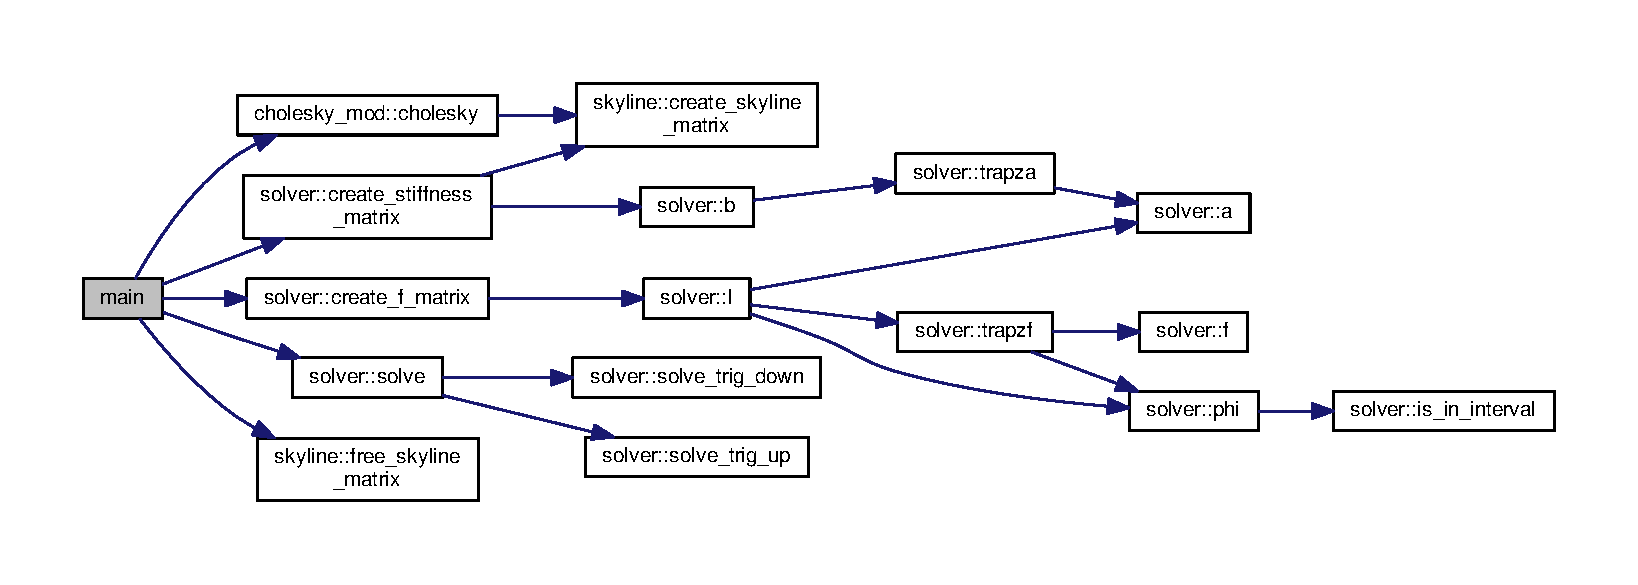
\includegraphics[width=350pt]{main_8f90_a8ec2266d83cd6c0b762cbcbc92c0af3d_cgraph}
\end{center}
\end{figure}

\hypertarget{_s_k_y_l_i_n_e_8f90}{}\section{src/\+S\+K\+Y\+L\+I\+NE.f90 File Reference}
\label{_s_k_y_l_i_n_e_8f90}\index{src/\+S\+K\+Y\+L\+I\+N\+E.\+f90@{src/\+S\+K\+Y\+L\+I\+N\+E.\+f90}}
\subsection*{Data Types}
\begin{DoxyCompactItemize}
\item 
type \hyperlink{structskyline_1_1skyline__matrix}{skyline\+::skyline\+\_\+matrix}
\end{DoxyCompactItemize}
\subsection*{Modules}
\begin{DoxyCompactItemize}
\item 
module \hyperlink{namespaceskyline}{skyline}
\begin{DoxyCompactList}\small\item\em Ce module permet de stocker une matrice sous la forme d\textquotesingle{}une matrice Skyline (profil) \end{DoxyCompactList}\end{DoxyCompactItemize}
\subsection*{Functions/\+Subroutines}
\begin{DoxyCompactItemize}
\item 
type(skyline\+\_\+matrix) function \hyperlink{namespaceskyline_a5fe1d351df2e3a07f96028d1d2a892a8}{skyline\+::create\+\_\+skyline\+\_\+matrix} (m, n)
\begin{DoxyCompactList}\small\item\em Créé une matrice S\+K\+Y\+L\+I\+NE vide de dimension $(m,n)$. \end{DoxyCompactList}\item 
type(skyline\+\_\+matrix) function \hyperlink{namespaceskyline_a86a4fe28bc106ef42d25cf7596c108bf}{skyline\+::create\+\_\+skyline\+\_\+matrix\+\_\+from\+\_\+file} (filename)
\begin{DoxyCompactList}\small\item\em Créé une matrice S\+K\+Y\+L\+I\+NE depuis les données contenus dans un fichier. \end{DoxyCompactList}\item 
subroutine \hyperlink{namespaceskyline_a3377a8391ad2d61659689fc8c4130bdc}{skyline\+::write\+\_\+skyline\+\_\+matrix\+\_\+to\+\_\+file} (M, filename)
\begin{DoxyCompactList}\small\item\em Sauvegarde une matrice S\+K\+Y\+L\+I\+NE dans un fichier. \end{DoxyCompactList}\item 
subroutine \hyperlink{namespaceskyline_a583c70b26e3bcb37ecb679f5c11ec2f4}{skyline\+::free\+\_\+skyline\+\_\+matrix} (M)
\begin{DoxyCompactList}\small\item\em Supprime les allocations mémoires d\textquotesingle{}une matrice S\+K\+Y\+L\+I\+NE. \end{DoxyCompactList}\item 
real function \hyperlink{namespaceskyline_a28077ec6714b830771f90da1b674b0ce}{skyline\+::get} (M, row, col)
\begin{DoxyCompactList}\small\item\em Accède aux éléments d\textquotesingle{}une matrice S\+K\+Y\+L\+I\+NE. \end{DoxyCompactList}\item 
integer function \hyperlink{namespaceskyline_a25b1e027d99abb67ab844d7b657a5843}{skyline\+::position\+\_\+on\+\_\+s} (M, row, col)
\begin{DoxyCompactList}\small\item\em Calcule la position d\textquotesingle{}un élément dans le tableau stockant les données. \end{DoxyCompactList}\item 
integer function \hyperlink{namespaceskyline_a9f07218be321c12bea1d84f6b629e346}{skyline\+::number\+\_\+item\+\_\+on\+\_\+line} (M, row)
\begin{DoxyCompactList}\small\item\em Calcule le nombre d\textquotesingle{}élément stocké sur une ligne. \end{DoxyCompactList}\item 
subroutine \hyperlink{namespaceskyline_a428818245223fbf6e3a5a2264f8f1a65}{skyline\+::display} (M)
\begin{DoxyCompactList}\small\item\em Affiche une matrice S\+K\+Y\+L\+I\+NE. \end{DoxyCompactList}\item 
subroutine \hyperlink{namespaceskyline_aedb0d55aecd5f4cae4dc3593a5e89f0f}{skyline\+::display\+\_\+debug} (M)
\begin{DoxyCompactList}\small\item\em Affiche des informations de debuguage d\textquotesingle{}une matrice S\+K\+Y\+L\+I\+NE. \end{DoxyCompactList}\item 
real function, dimension(\+:), allocatable \hyperlink{namespaceskyline_ae156a973c4a30bd2740af6ef2fdfa1d9}{skyline\+::prod\+\_\+mat\+\_\+vec} (M, X)
\begin{DoxyCompactList}\small\item\em Calcule Le produit entre une matrice et un vecteur. \end{DoxyCompactList}\end{DoxyCompactItemize}

\hypertarget{_s_o_l_v_e_r_8f90}{}\section{Référence du fichier src/\+S\+O\+L\+V\+ER.f90}
\label{_s_o_l_v_e_r_8f90}\index{src/\+S\+O\+L\+V\+E\+R.\+f90@{src/\+S\+O\+L\+V\+E\+R.\+f90}}
\subsection*{Modules}
\begin{DoxyCompactItemize}
\item 
module \hyperlink{namespacesolver}{solver}
\begin{DoxyCompactList}\small\item\em Ce module permet de résoudre un problème d\textquotesingle{}éléments fini. \end{DoxyCompactList}\end{DoxyCompactItemize}
\subsection*{Fonctions/\+Subroutines}
\begin{DoxyCompactItemize}
\item 
real function \hyperlink{namespacesolver_ab0081bb7880652eb26e65994f13fcb54}{solver\+::a} (x)
\begin{DoxyCompactList}\small\item\em Fonction A(x) du problème donné \end{DoxyCompactList}\item 
real function \hyperlink{namespacesolver_a6f4d43c88c7c8ebdea64bd45e002af05}{solver\+::f} (x)
\begin{DoxyCompactList}\small\item\em Fonction F(x) du problème donné \end{DoxyCompactList}\item 
logical function \hyperlink{namespacesolver_a2380e35eaa6fcef040f90bb5b23baa6a}{solver\+::is\+\_\+in\+\_\+interval} (x, xmin, xmax)
\begin{DoxyCompactList}\small\item\em Calcule si une valeur est dans un intervalle donné \end{DoxyCompactList}\item 
real function \hyperlink{namespacesolver_a3323b7ad7f72685a465733177c82e8cc}{solver\+::phi} (i, x, h, Xdiscret)
\begin{DoxyCompactList}\small\item\em Fonction de base. \end{DoxyCompactList}\item 
real function \hyperlink{namespacesolver_add1e5803b09e373fde46731960030e42}{solver\+::phi\+\_\+der} (i, x, h, Xdiscret)
\begin{DoxyCompactList}\small\item\em Dérivée de la fonction de base. \end{DoxyCompactList}\item 
real function \hyperlink{namespacesolver_a5cdc774a6979796cb6b072b2fbb0e5af}{solver\+::trapza} (binf, bsup, N)
\begin{DoxyCompactList}\small\item\em Calcul de l\textquotesingle{}intégrale du terme bilinéaire. \end{DoxyCompactList}\item 
real function \hyperlink{namespacesolver_adb6590794b23eaed708cd2e42adac550}{solver\+::trapzf} (binf, bsup, N, ix, hx, Xdiscret)
\begin{DoxyCompactList}\small\item\em Calcul de l\textquotesingle{}intégrale du terme Linéaire. \end{DoxyCompactList}\item 
real function \hyperlink{namespacesolver_a99565d1c8ed5142211b78fe3ccca060b}{solver\+::b} (i, j, h, Xdiscret, Nitg)
\begin{DoxyCompactList}\small\item\em Evaluation du terme bilinéaire. \end{DoxyCompactList}\item 
real function \hyperlink{namespacesolver_a327c990a10263590618db7a31c4edcc9}{solver\+::l} (i, h, Xdiscret, Nitg, alpha1)
\begin{DoxyCompactList}\small\item\em Evaluation du terme Linéaire. \end{DoxyCompactList}\item 
type(skyline\+\_\+matrix) function \hyperlink{namespacesolver_aefd2f88bd66b9d9ccce170259a49c77d}{solver\+::create\+\_\+stiffness\+\_\+matrix} (h, Xdiscret, Nitg)
\begin{DoxyCompactList}\small\item\em Calcul la matrice de rigidité \end{DoxyCompactList}\item 
real function, dimension(\+:), allocatable \hyperlink{namespacesolver_af45a5f246a818112e6a257335c2b829d}{solver\+::create\+\_\+f\+\_\+matrix} (h, Xdiscret, Nitg, alpha1)
\begin{DoxyCompactList}\small\item\em Calcule du second membre. \end{DoxyCompactList}\item 
real function, dimension(\+:), allocatable \hyperlink{namespacesolver_ad8b8ef6c982475b3fb276f93660b750f}{solver\+::solve\+\_\+trig\+\_\+down} (LT, BB)
\begin{DoxyCompactList}\small\item\em Résouds le système triangulaire inférieur. \end{DoxyCompactList}\item 
real function, dimension(\+:), allocatable \hyperlink{namespacesolver_a08b8f70c86d7bf39b32ce8fdcc872fd4}{solver\+::solve\+\_\+trig\+\_\+up} (LT, BB)
\begin{DoxyCompactList}\small\item\em Résouds le système triangulaire supérieur. \end{DoxyCompactList}\item 
real function, dimension(\+:), allocatable \hyperlink{namespacesolver_af3691d2059a024a82bab7751a99e6006}{solver\+::solve} (LT, BB)
\begin{DoxyCompactList}\small\item\em Résouds le problème $ LT*Y = BB$. \end{DoxyCompactList}\end{DoxyCompactItemize}

%--- End generated contents ---

% Index
\backmatter
\newpage
\phantomsection
\clearemptydoublepage
\addcontentsline{toc}{chapter}{Index}
\printindex

\end{document}
